\section{Completed Demonstration Hardware Model}
This section presents the completed model of the project for demonstration. Each following will show the result of hardware design in previous sections, included the photo of real products and their layouts.
\begin{figure}[!htb]
    \begin{center}
    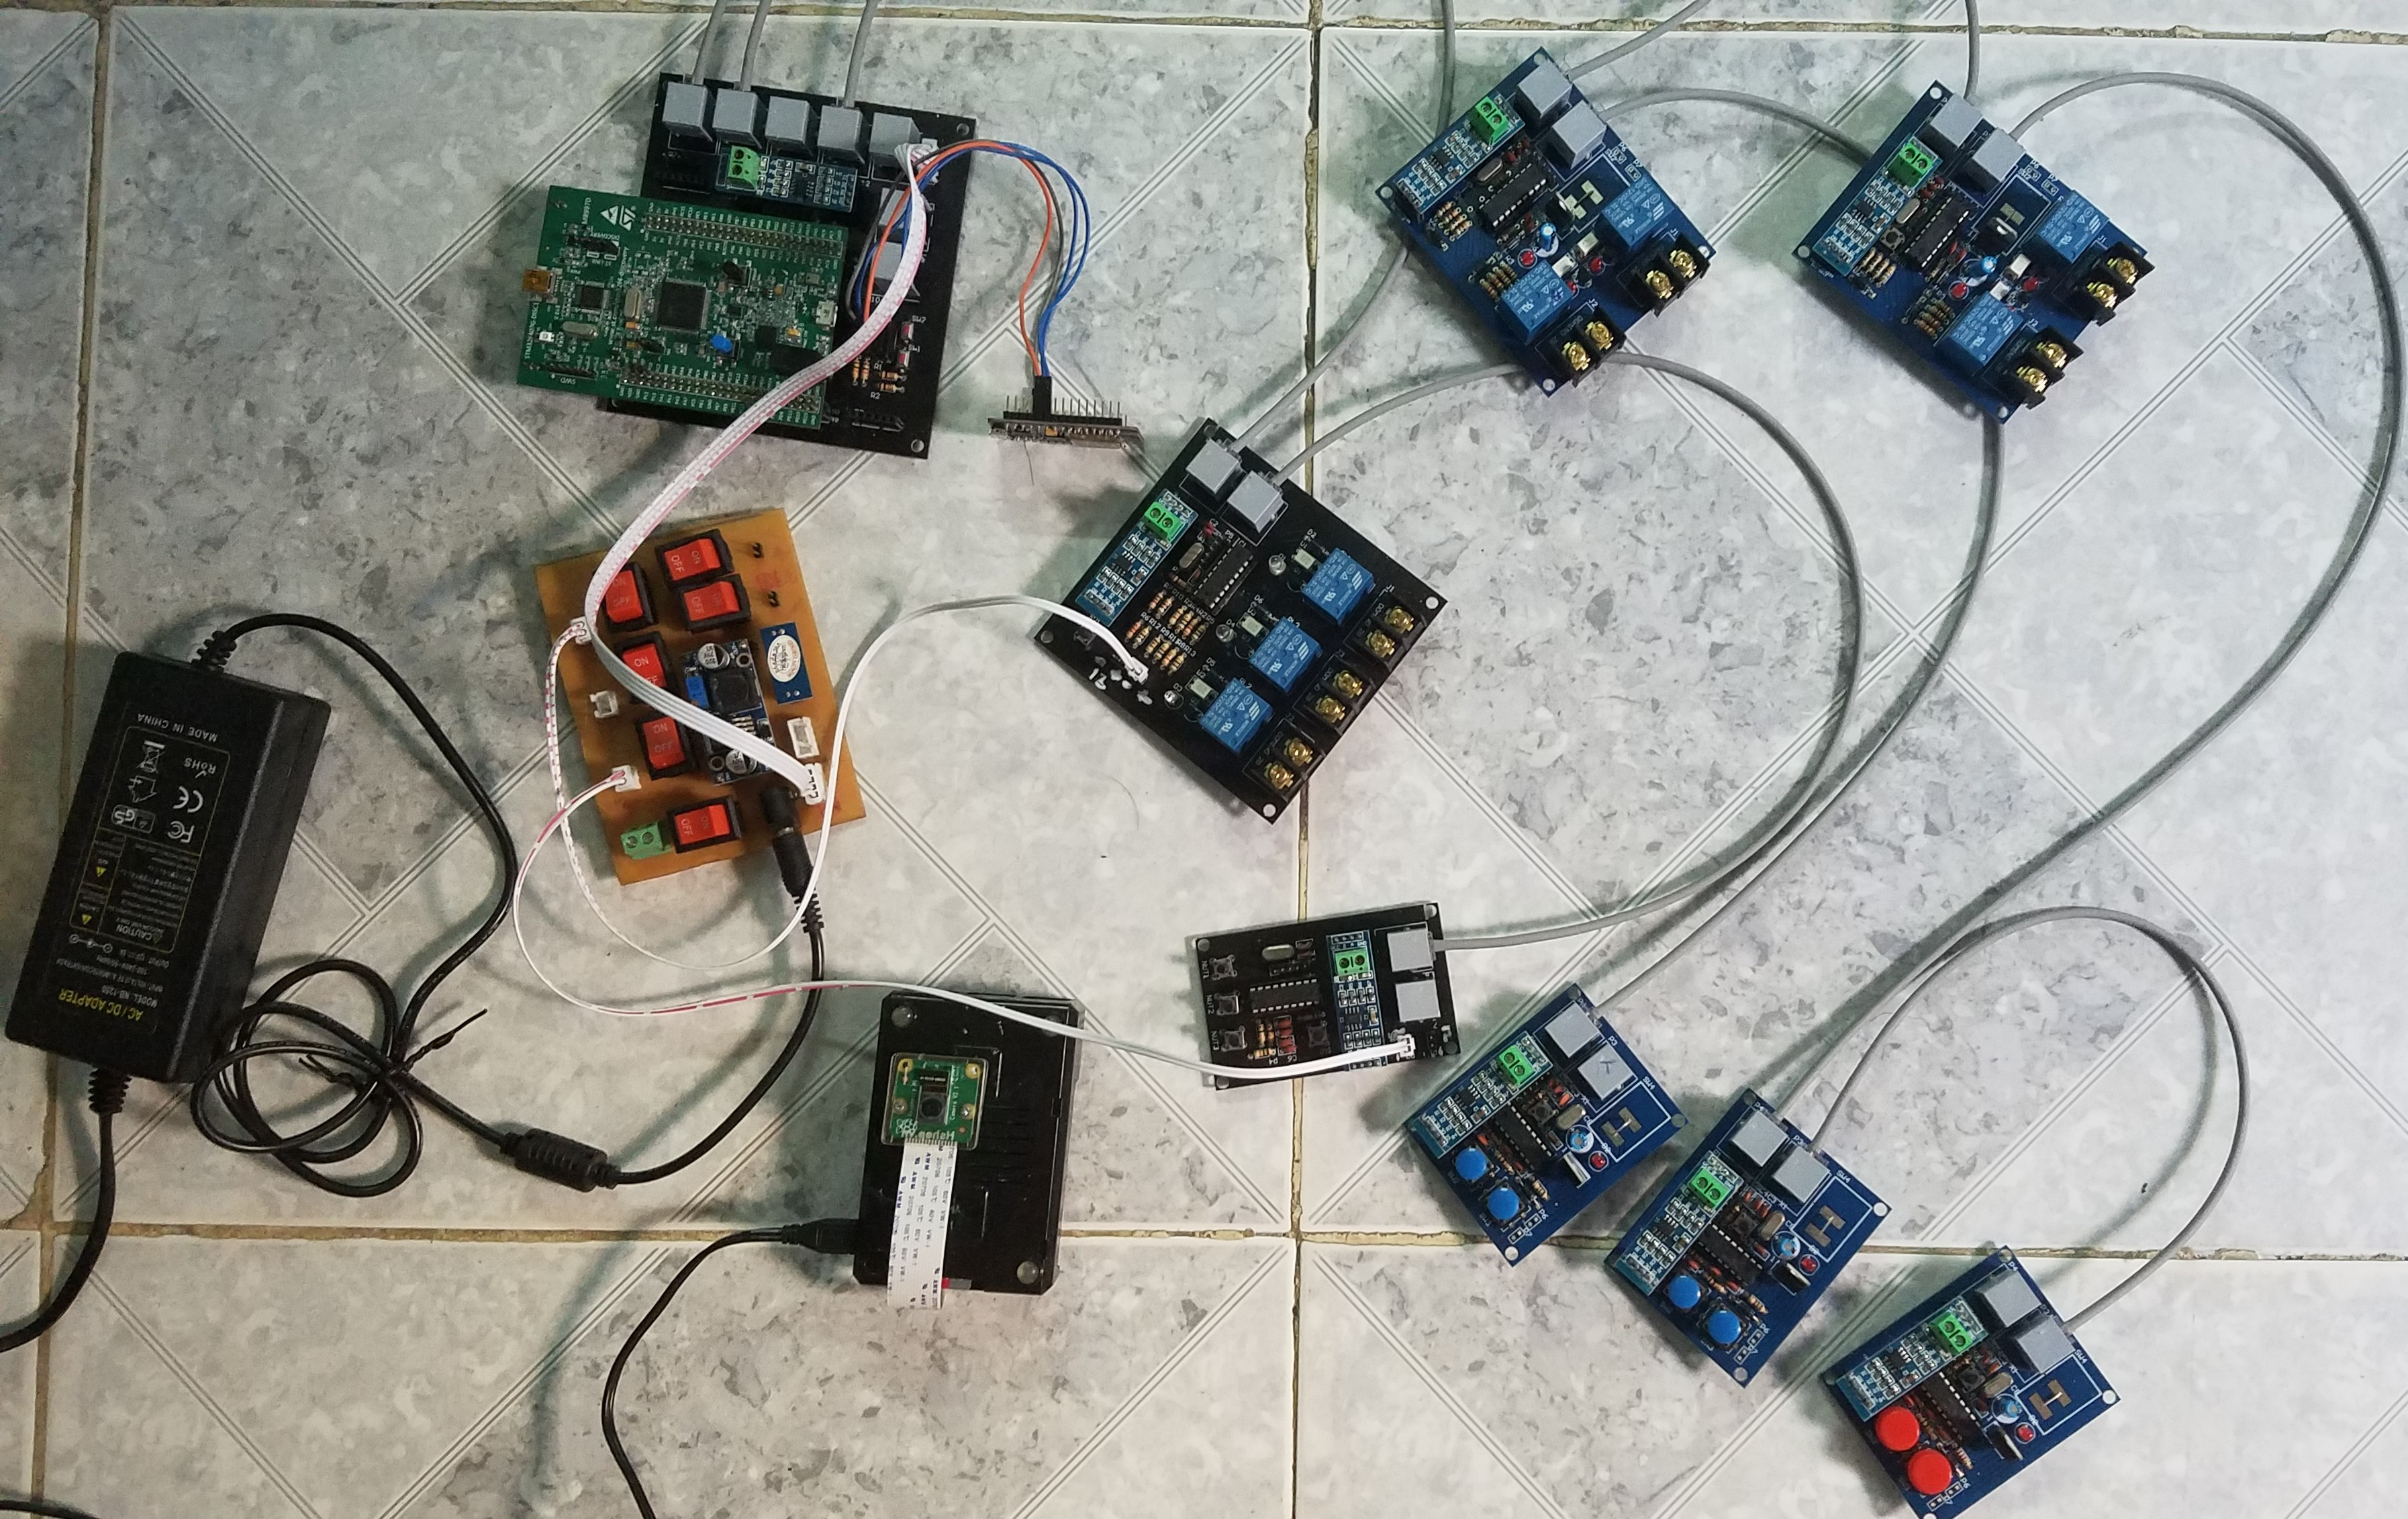
\includegraphics[scale=0.12]{images/overall.jpg}
    \caption{Completed Demonstration Model}
    \label{fig:completeDemo}
    \end{center}
\end{figure}

\section{Power for Master and the Slaves}
In this section, the author presents the Power for Master and the Slaves hardware in real circuits and also their layouts. The slaves are Slave 3 Buttons, Slave 2 Buttons, Slave 1 Button, Slave 3 Relays and Slave 2 Relays, respectively.
\begin{figure}[!htbp]
    \begin{center}
    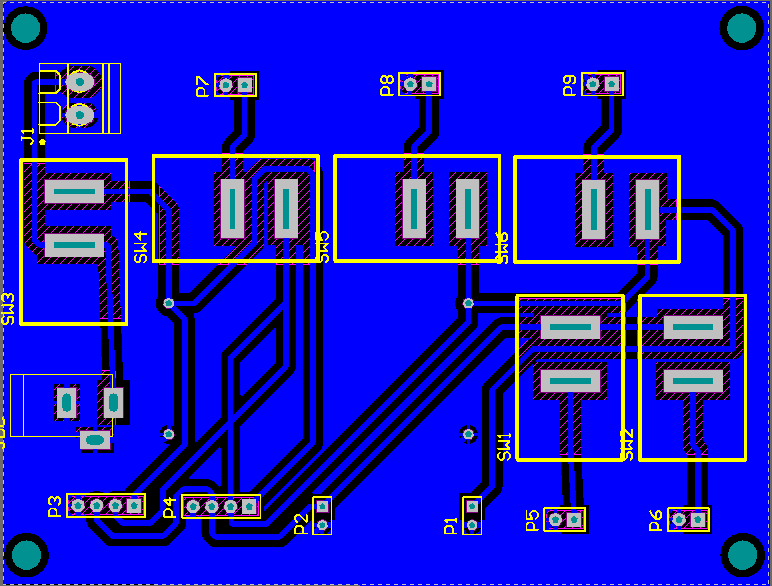
\includegraphics[scale=0.65]{images/powerLayout.png}\\

    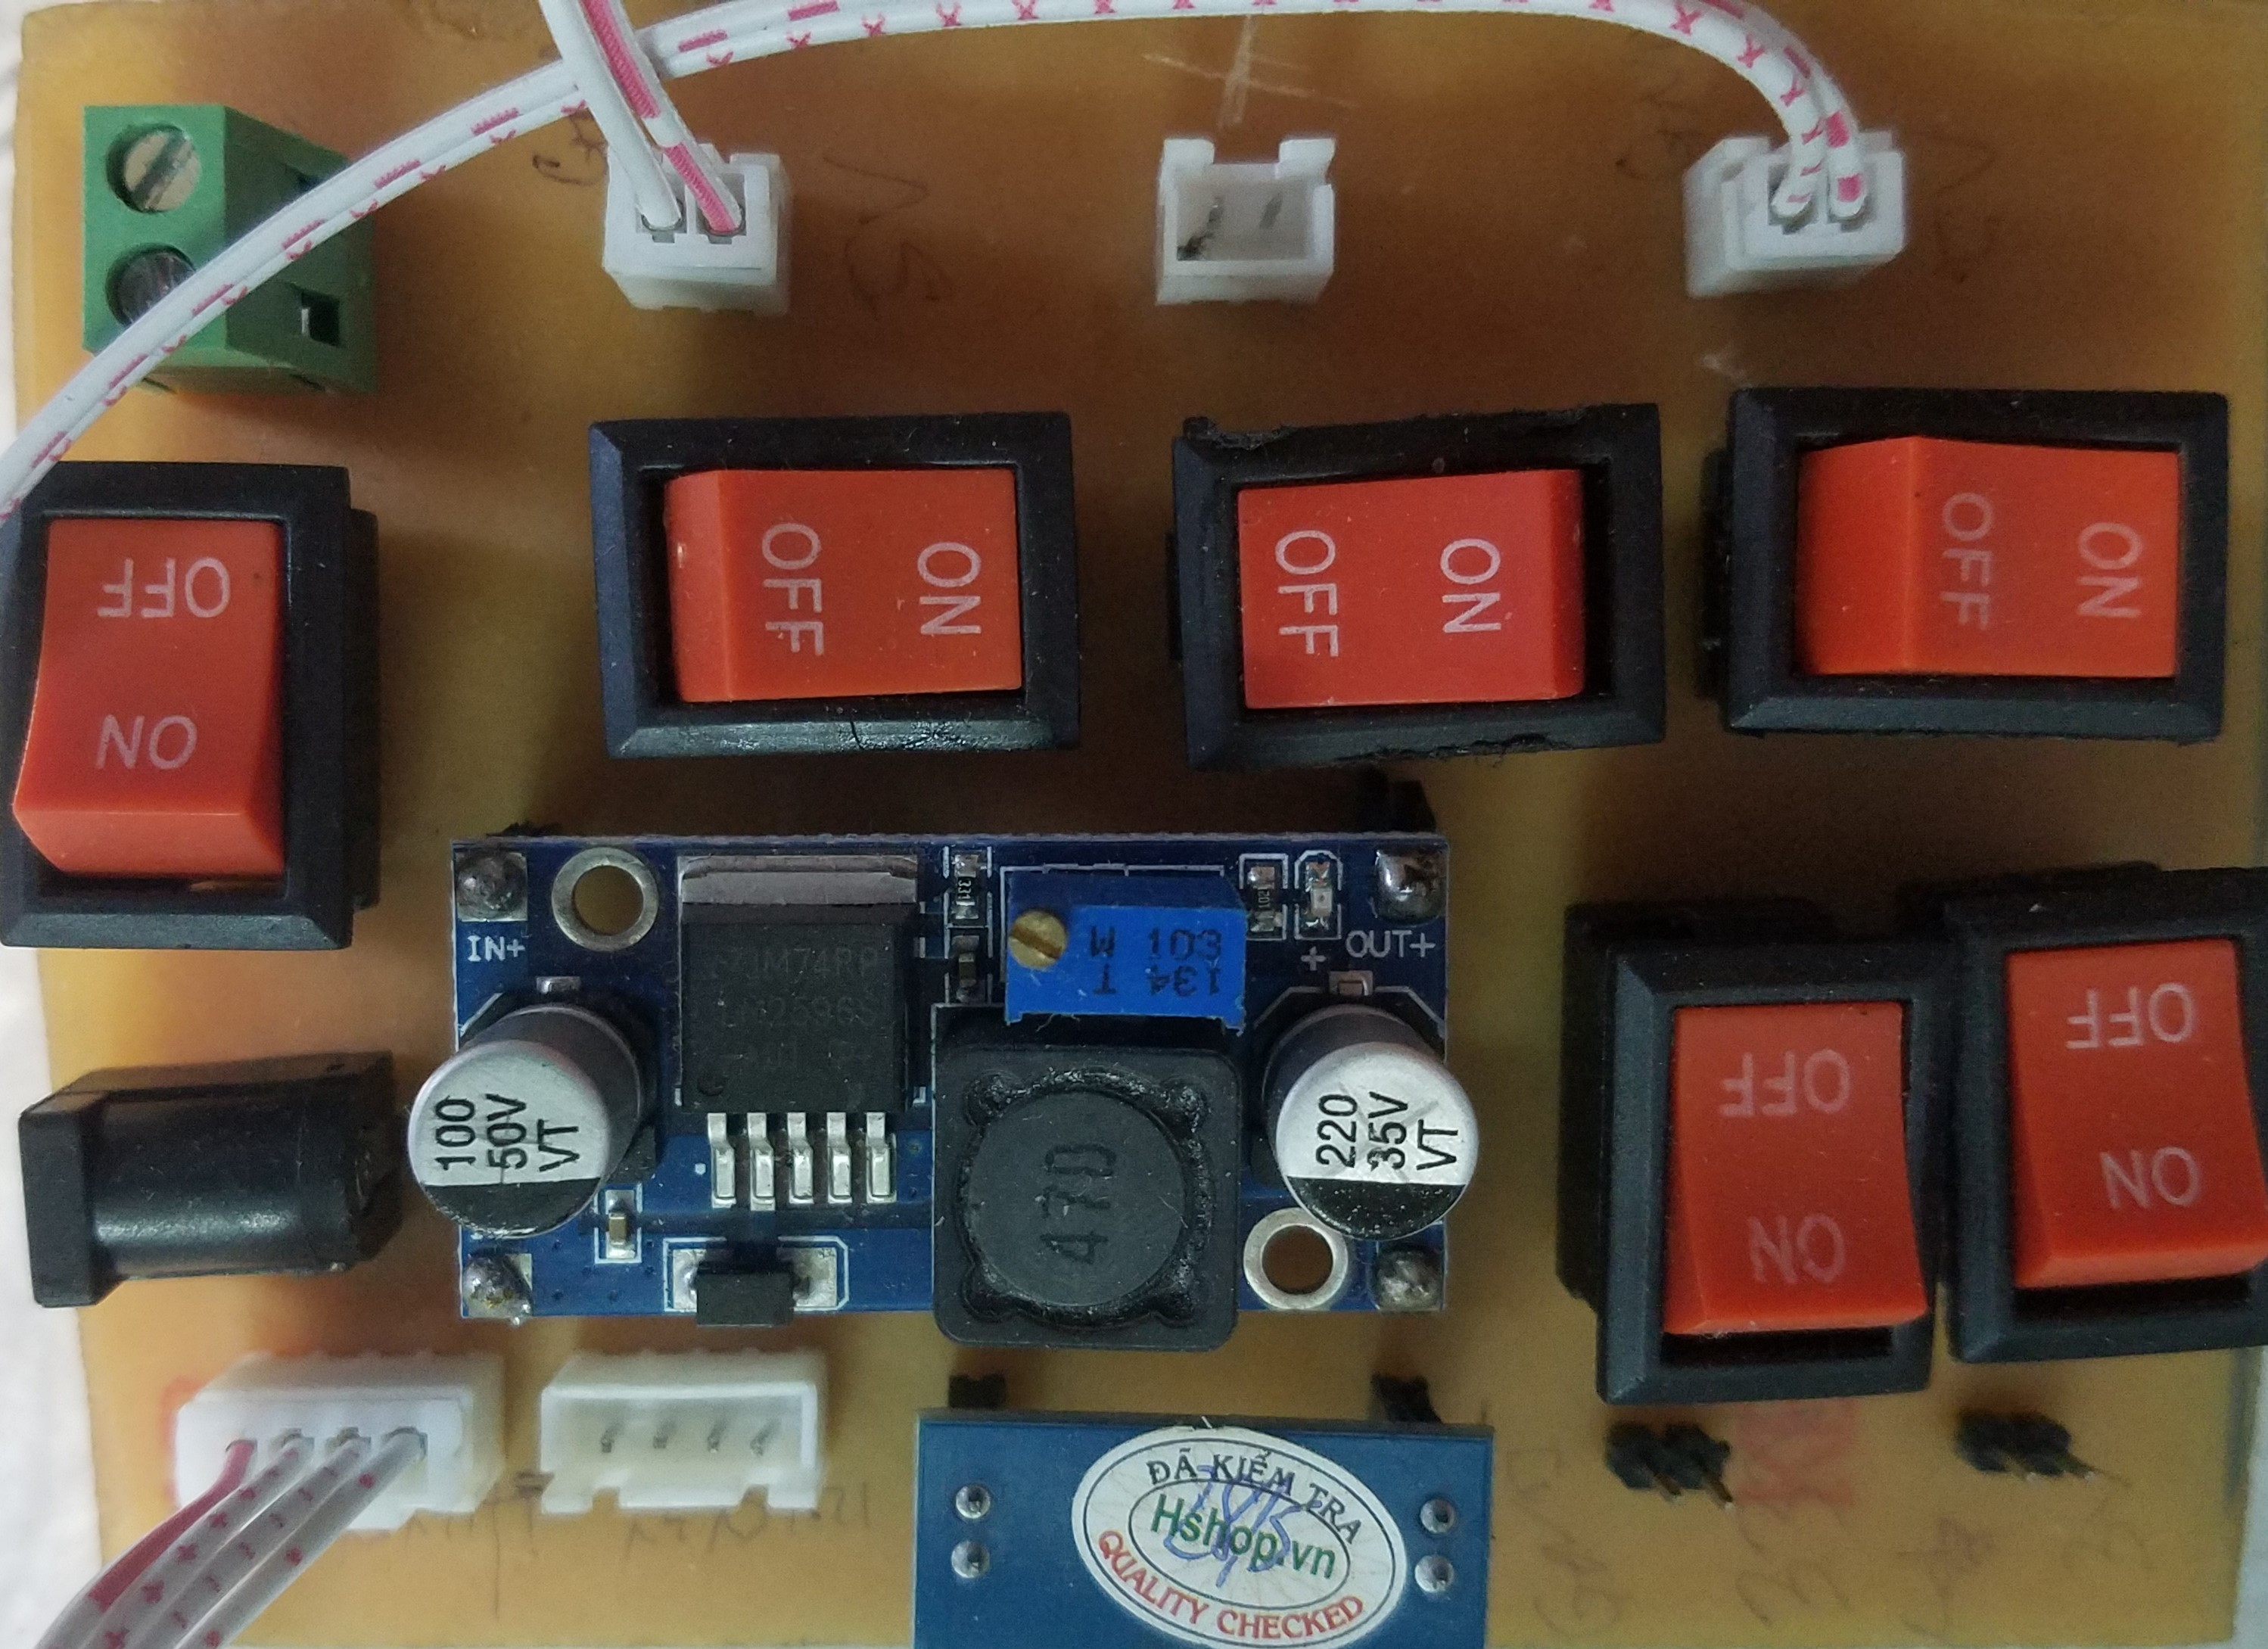
\includegraphics[scale=0.13]{images/power.jpg}
    \caption{Power for Master circuit}
    \label{fig:powerCircuit}
    \end{center}
\end{figure}
\begin{figure}[!htp]
    \begin{center}
    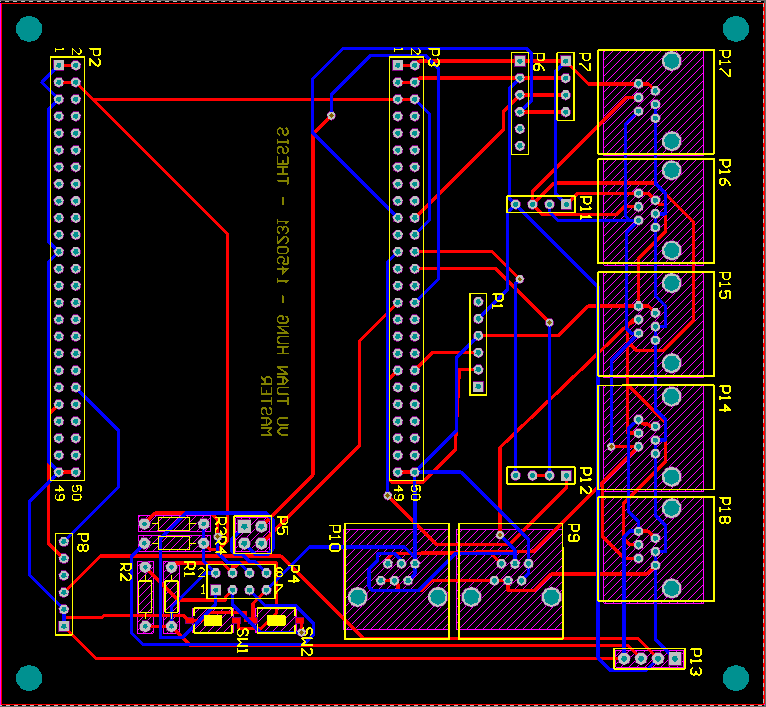
\includegraphics[scale=0.5]{images/masterLayout.png}\\

    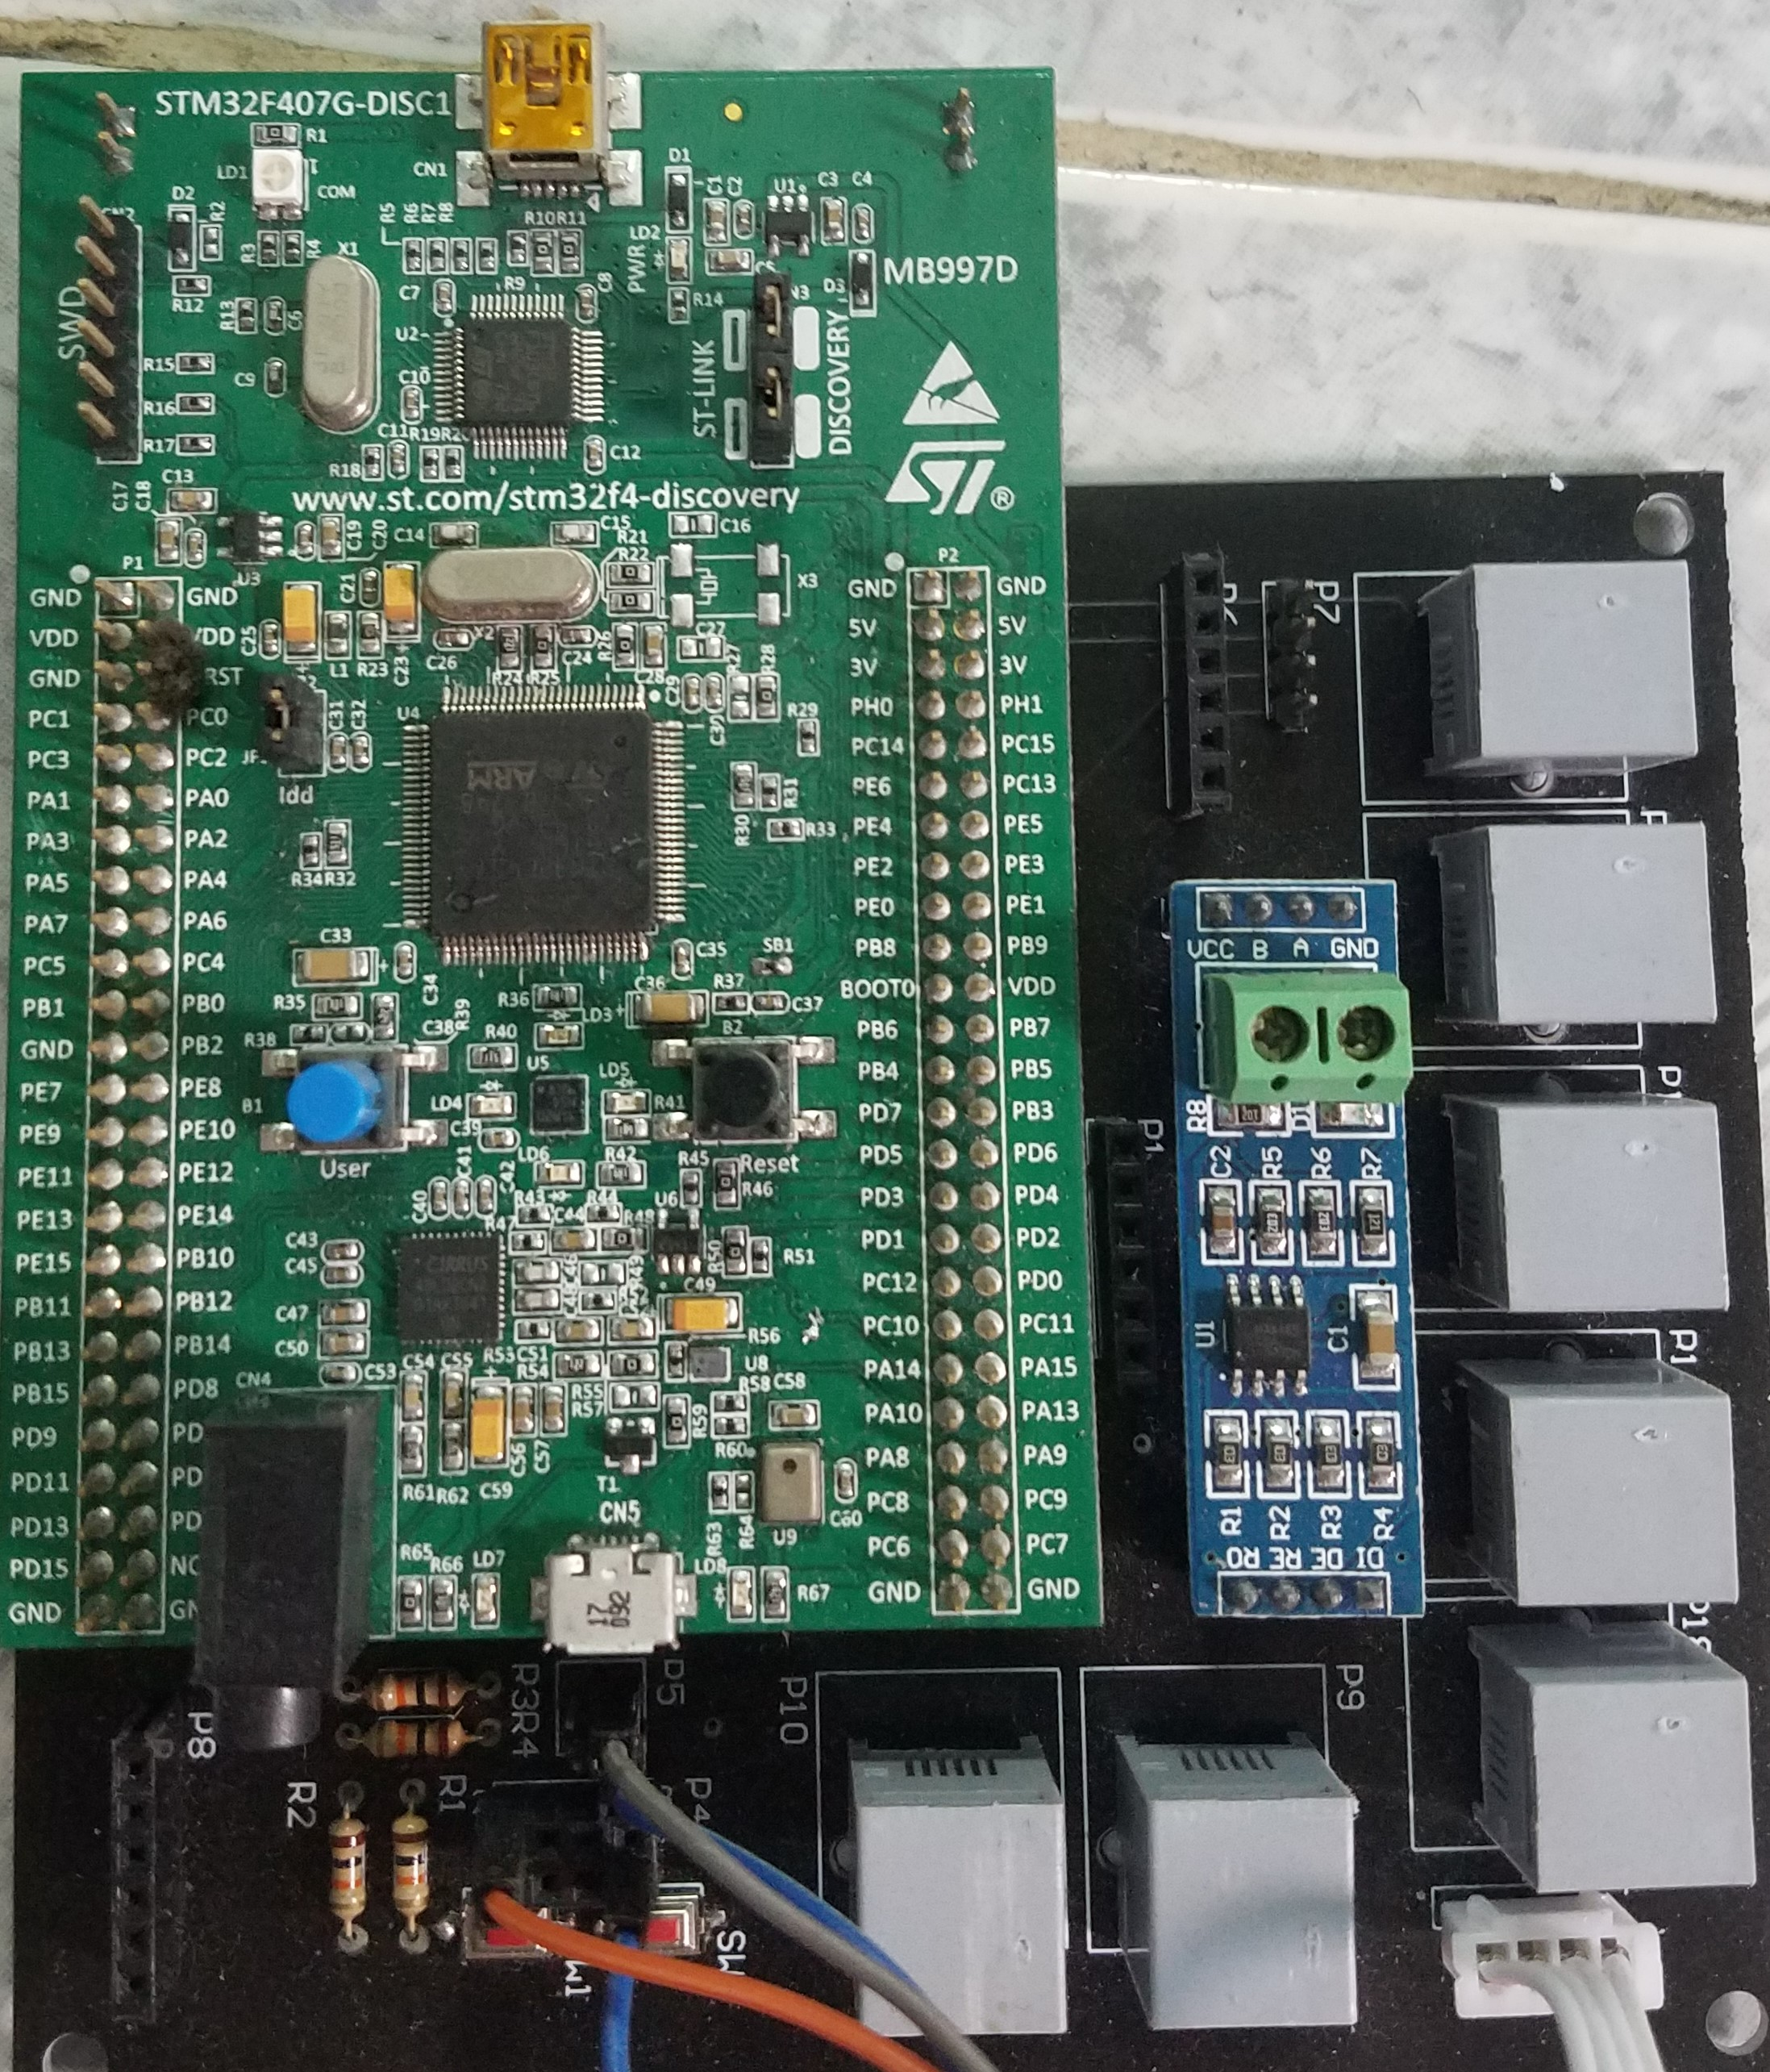
\includegraphics[scale=0.13]{images/m.jpg}
    \caption{Master circuit}
    \label{fig:masterCircuit}
    \end{center}
\end{figure}
\begin{figure}[!htbp]
    \begin{center}
    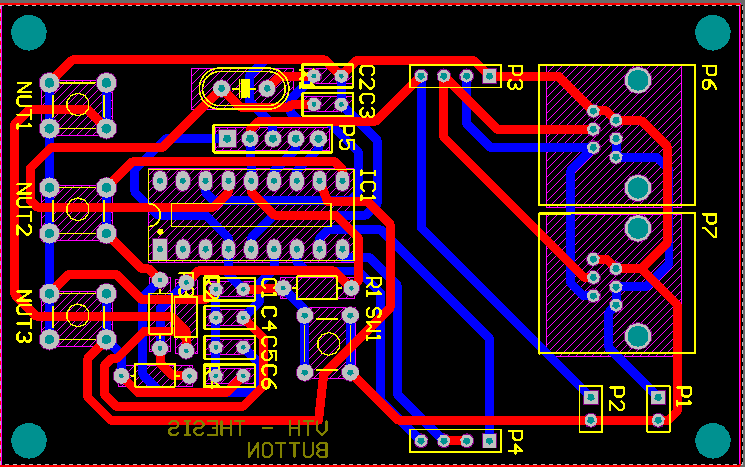
\includegraphics[scale=0.75]{images/s3bLayout.png}\\

    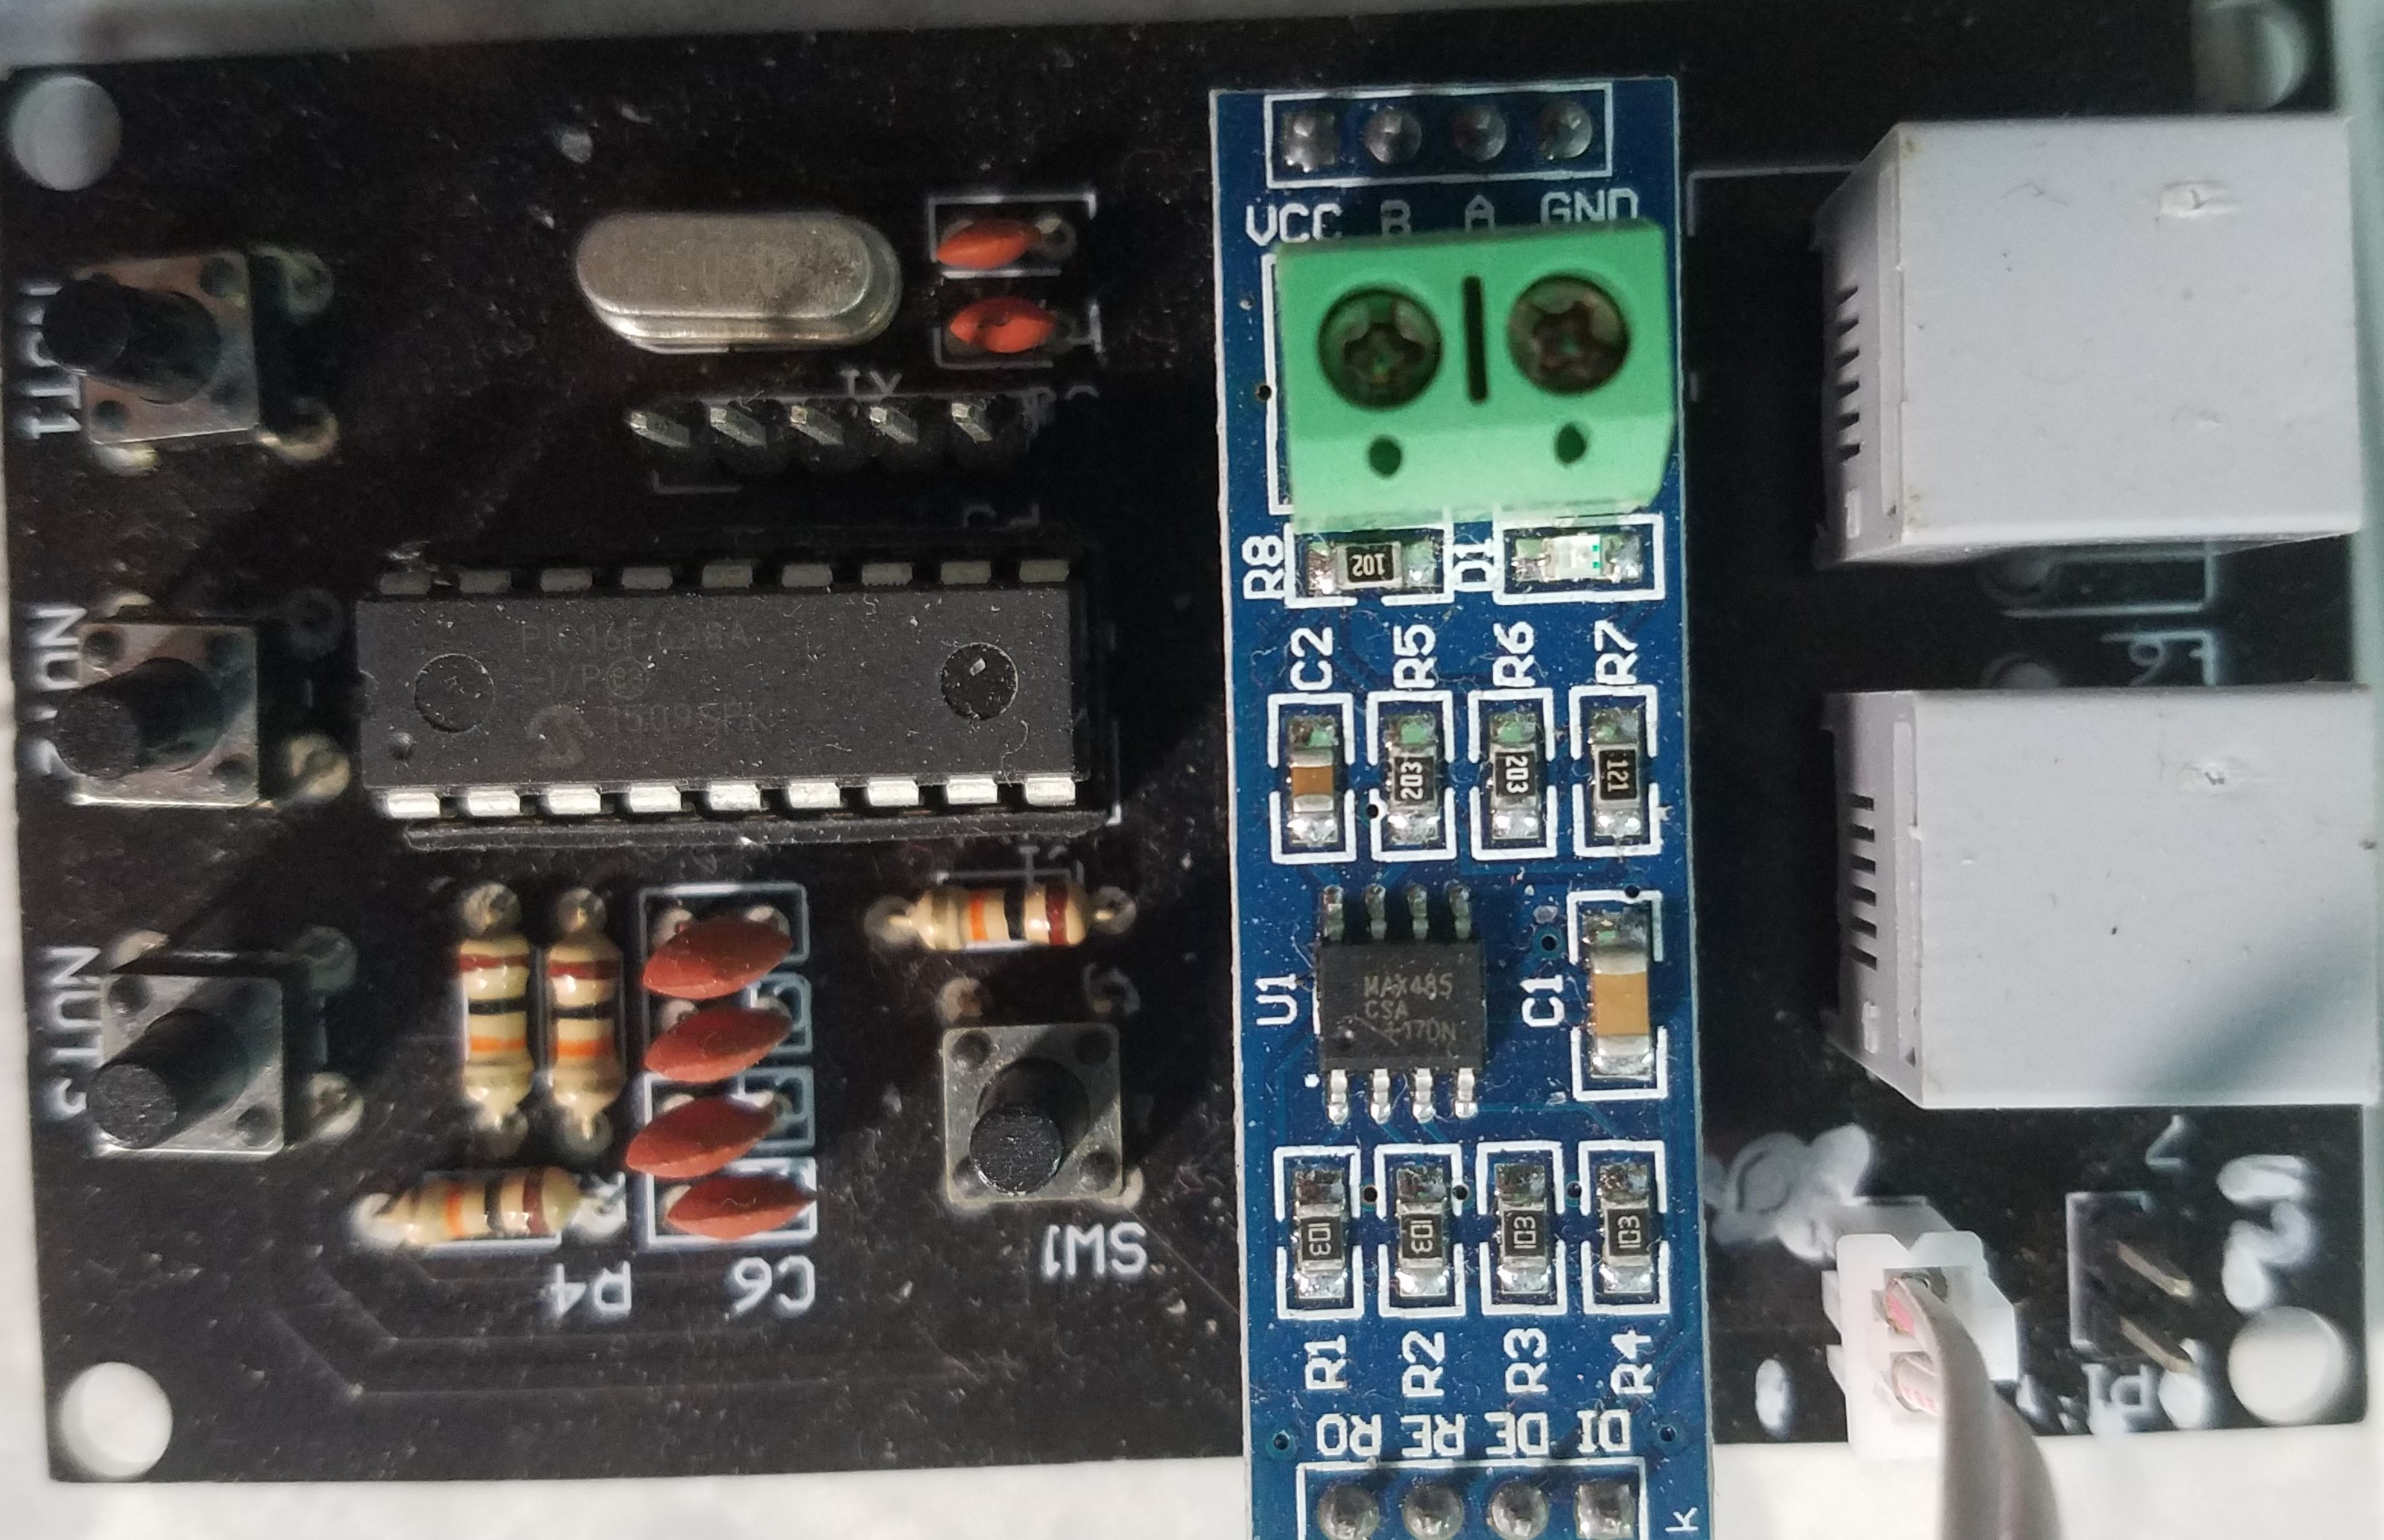
\includegraphics[scale=0.13]{images/s3b.jpg}
    \caption{Slave 3 Buttons circuit}
    \label{fig:slave3ButtonsCircuit}
    \end{center}
\end{figure}
\begin{figure}[!htbp]
    \begin{center}
    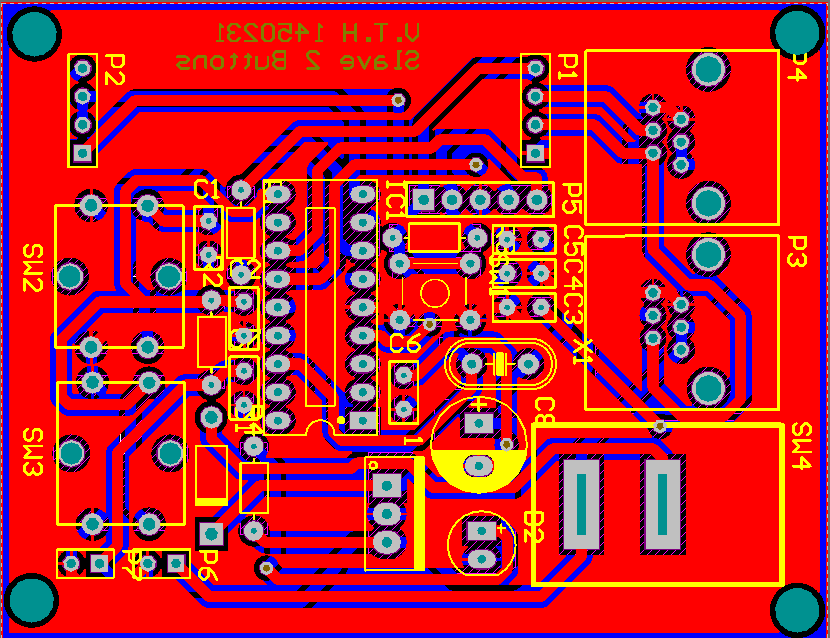
\includegraphics[scale=0.6]{images/s2bLayout.png}\\

    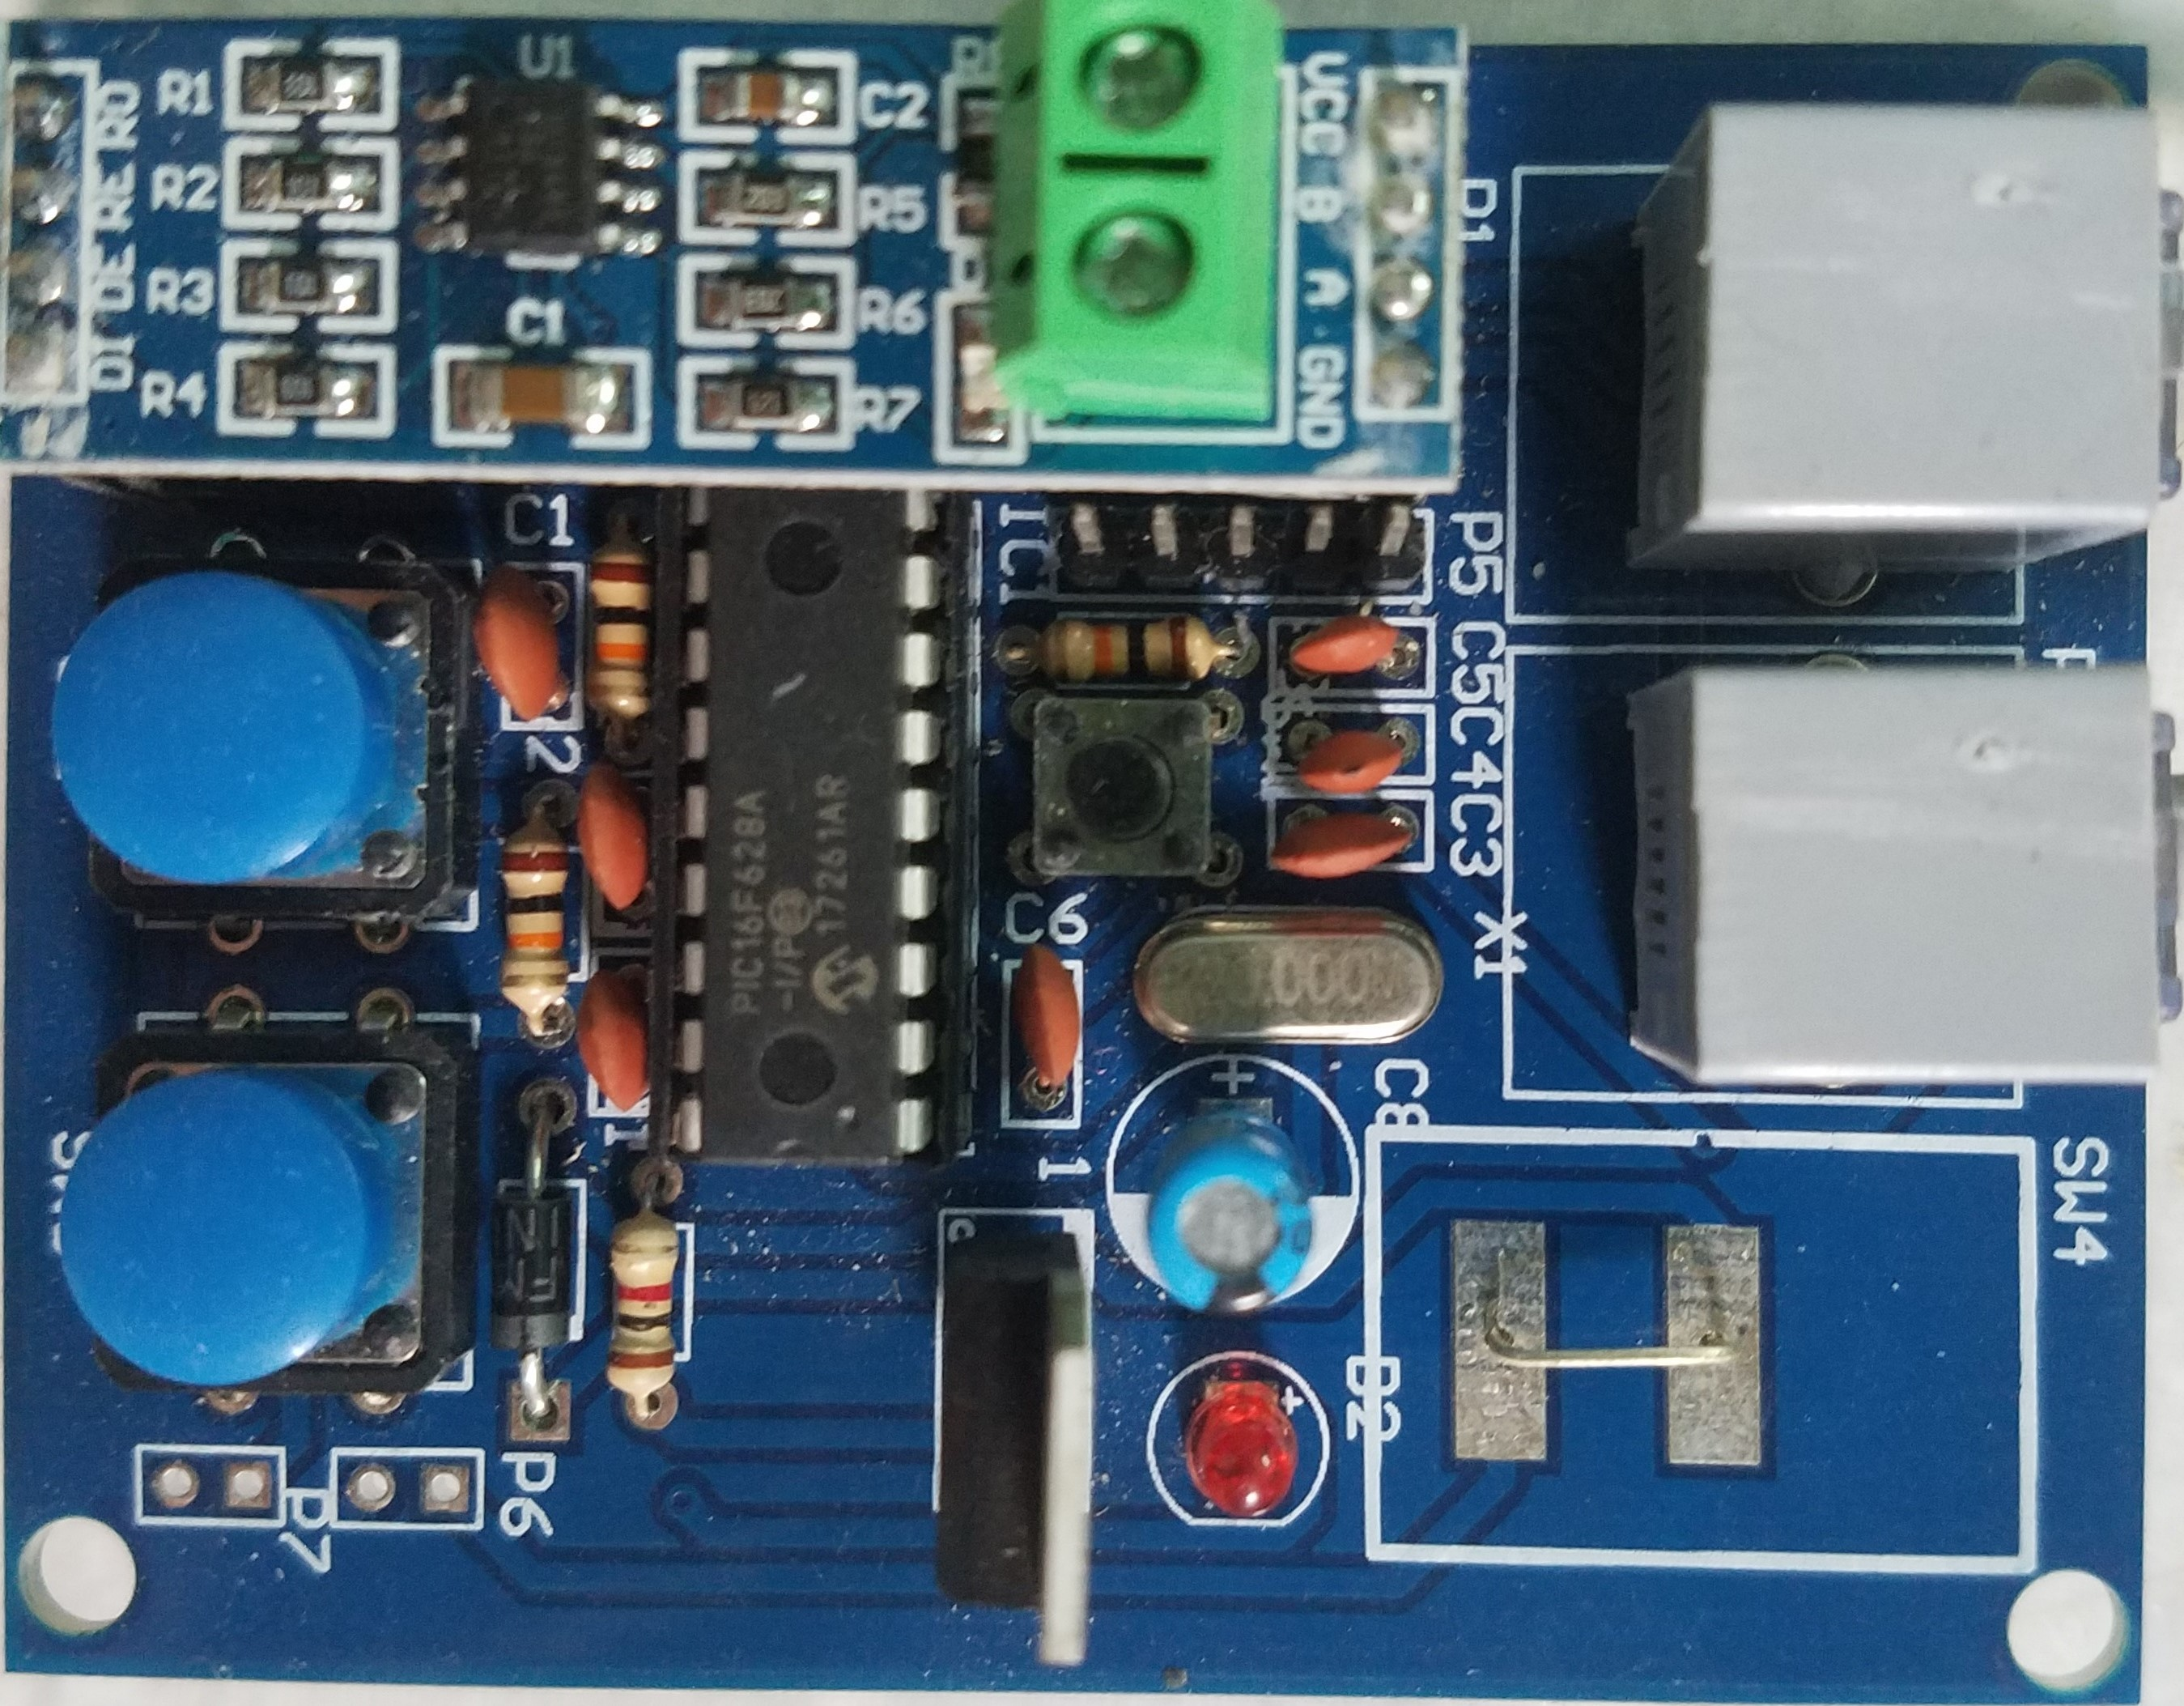
\includegraphics[scale=0.15]{images/s2b.jpg}
    \caption{Slave 2 Buttons circuit}
    \label{fig:slave2ButtonsCircuit}
    \end{center}
\end{figure}
\begin{figure}[!htbp]
    \begin{center}
    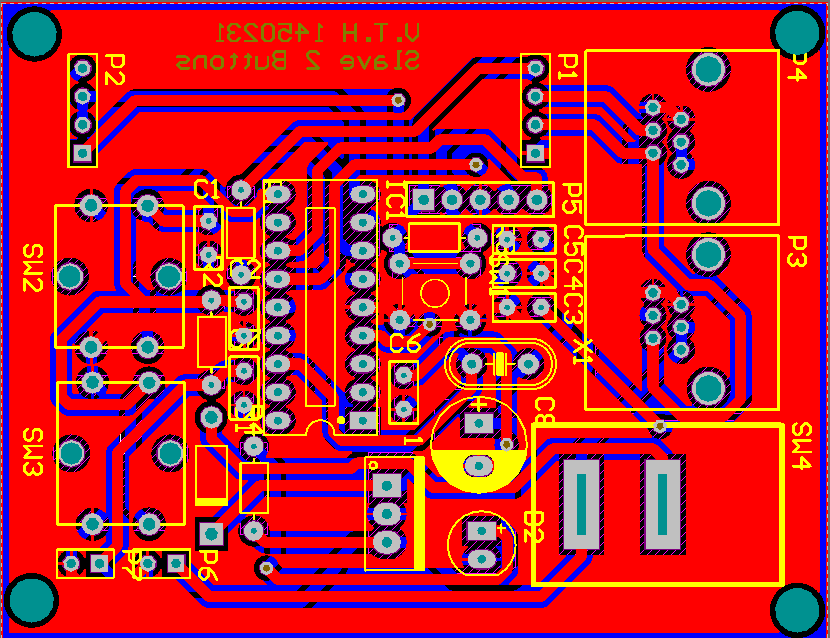
\includegraphics[scale=0.6]{images/s2bLayout.png}\\

    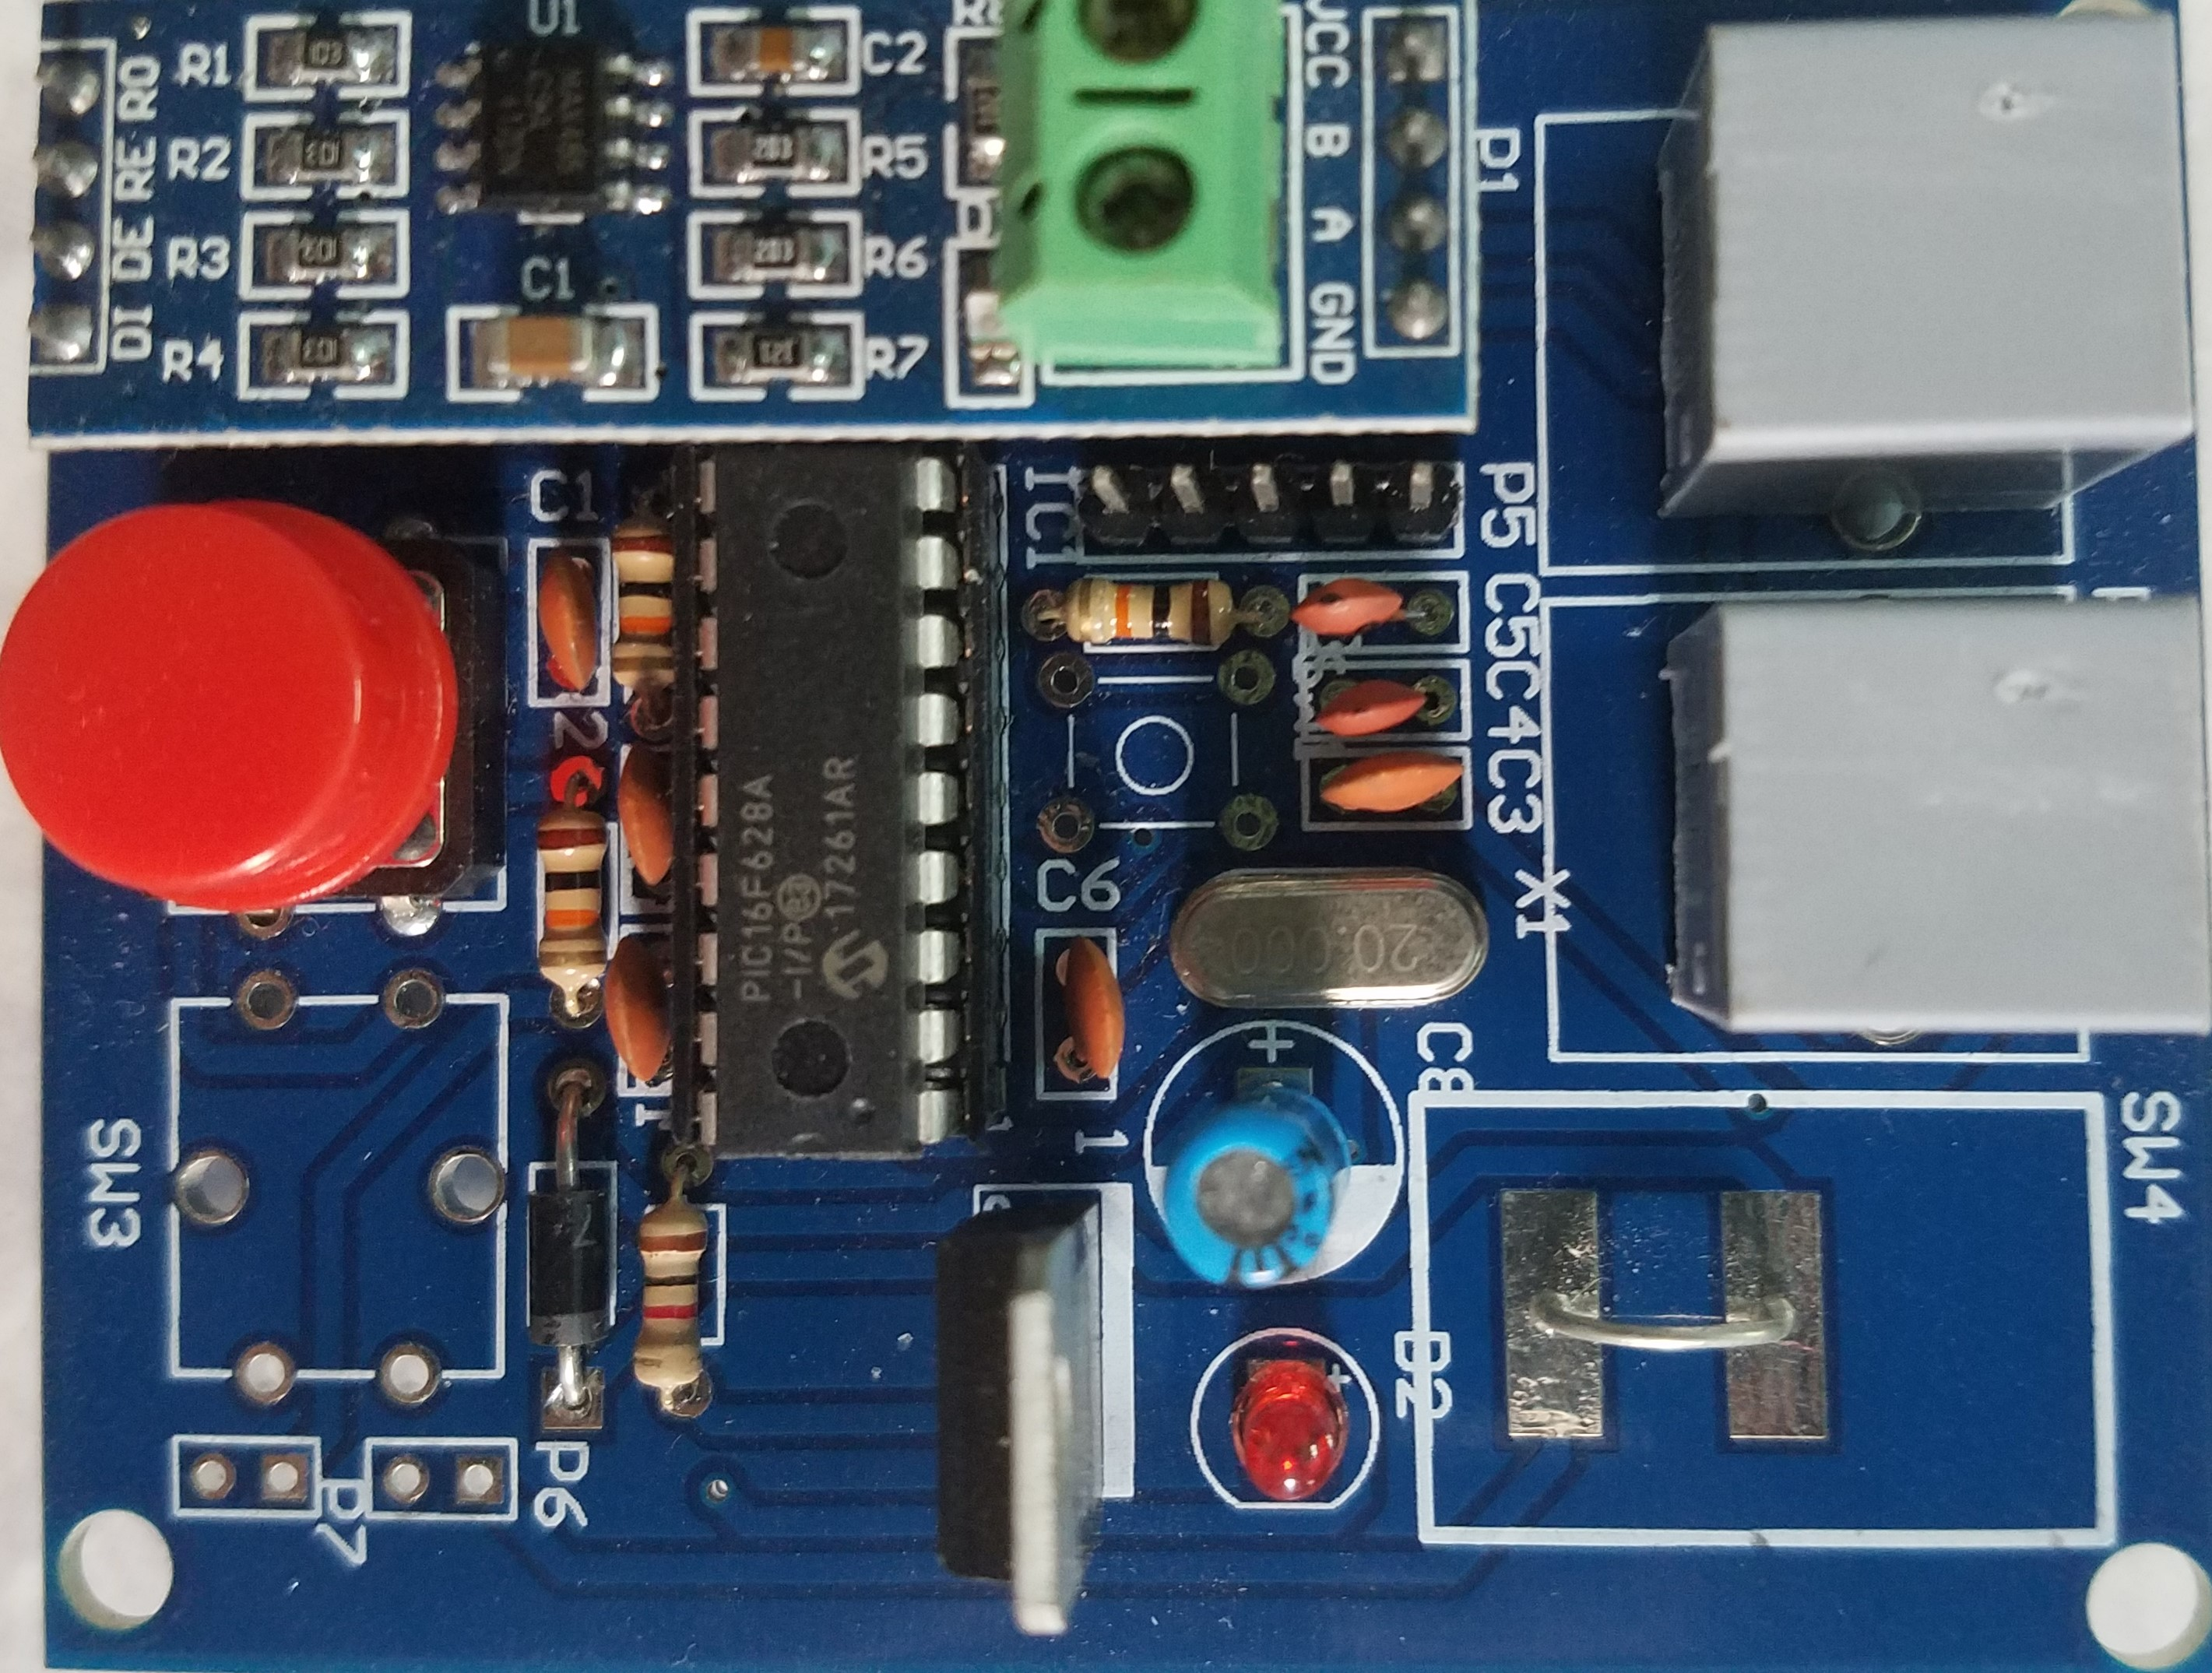
\includegraphics[scale=0.13]{images/s1b.jpg}
    \caption{Slave 1 Button circuit}
    \label{fig:slave1ButtonCircuit}
    \end{center}
\end{figure}
\begin{figure}[!htbp]
    \begin{center}
    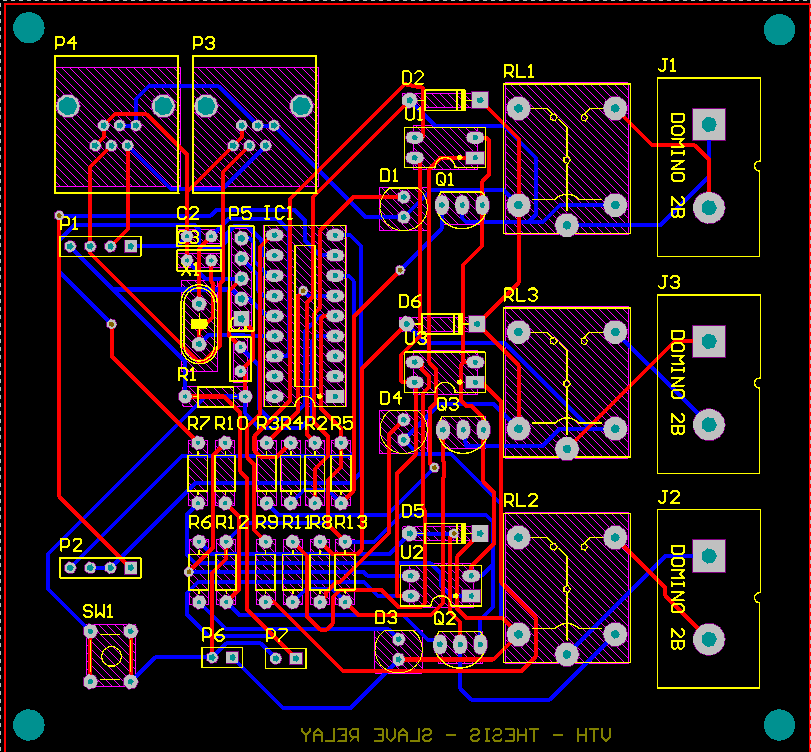
\includegraphics[scale=0.6]{images/s3rLayout.png}\\

    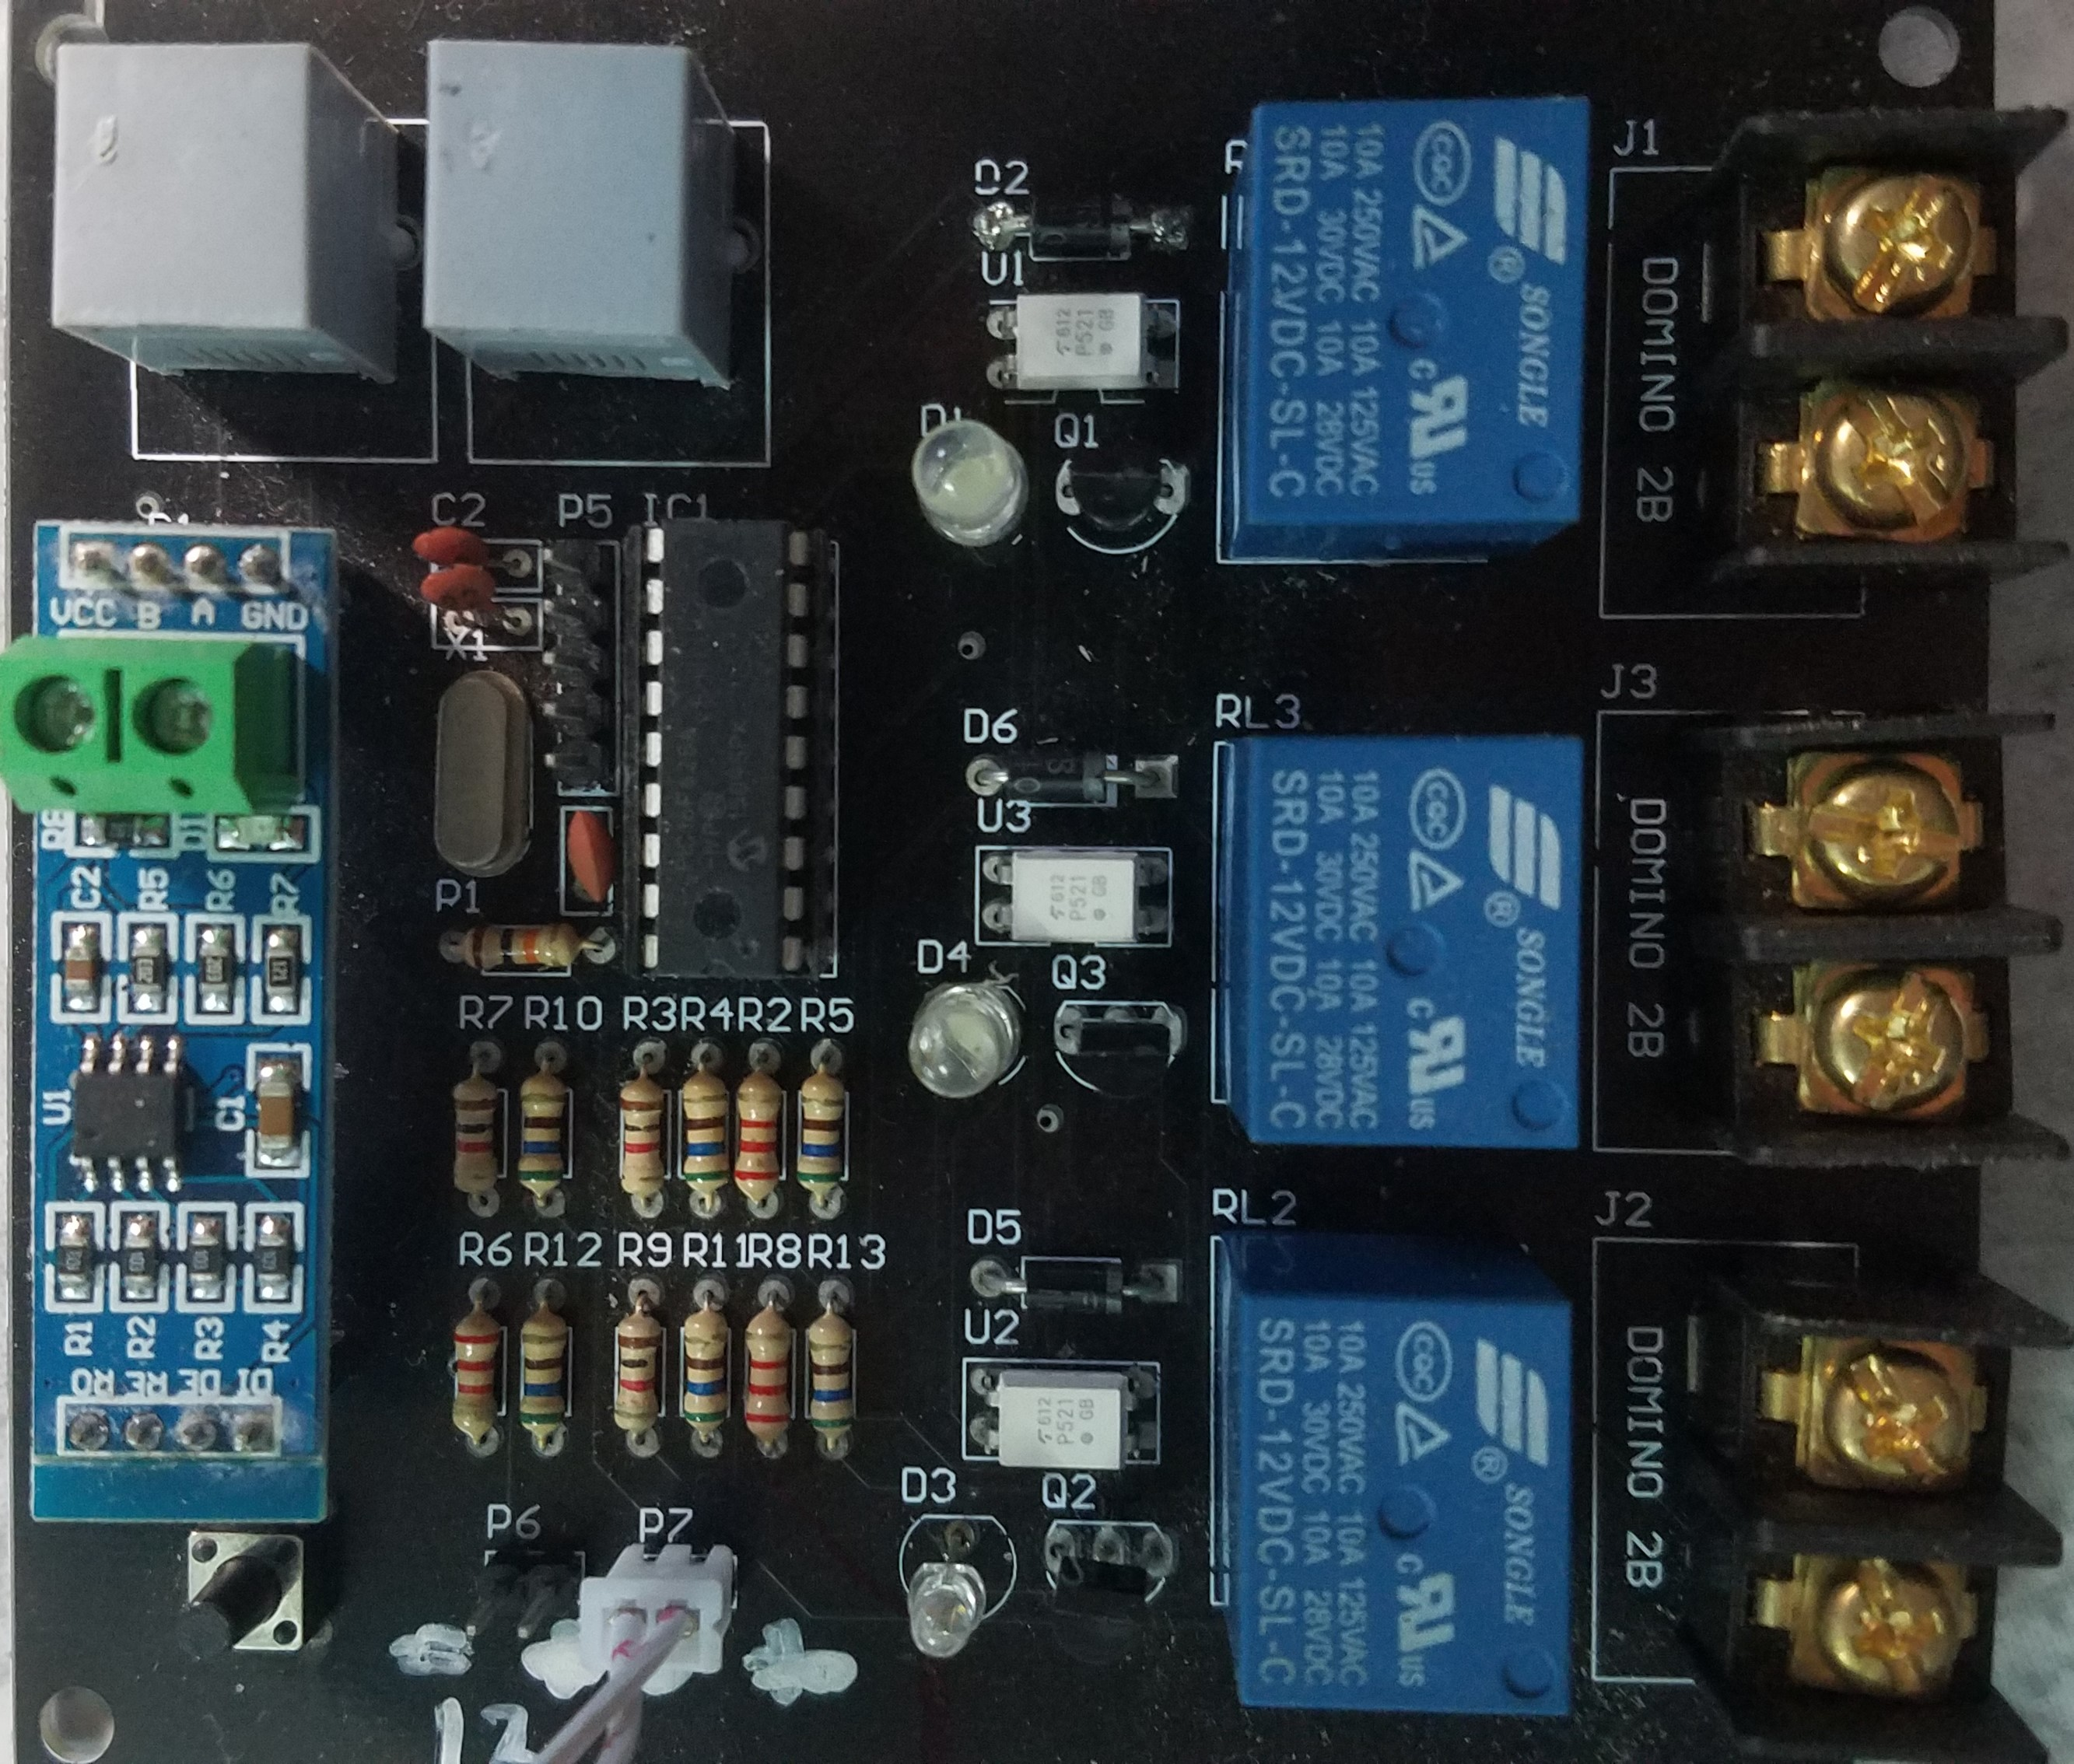
\includegraphics[scale=0.13]{images/s3r.jpg}
    \caption{Slave 3 Relays circuit}
    \label{fig:slave3RelaysCircuit}
    \end{center}
\end{figure}
\begin{figure}[!htbp]
    \begin{center}
    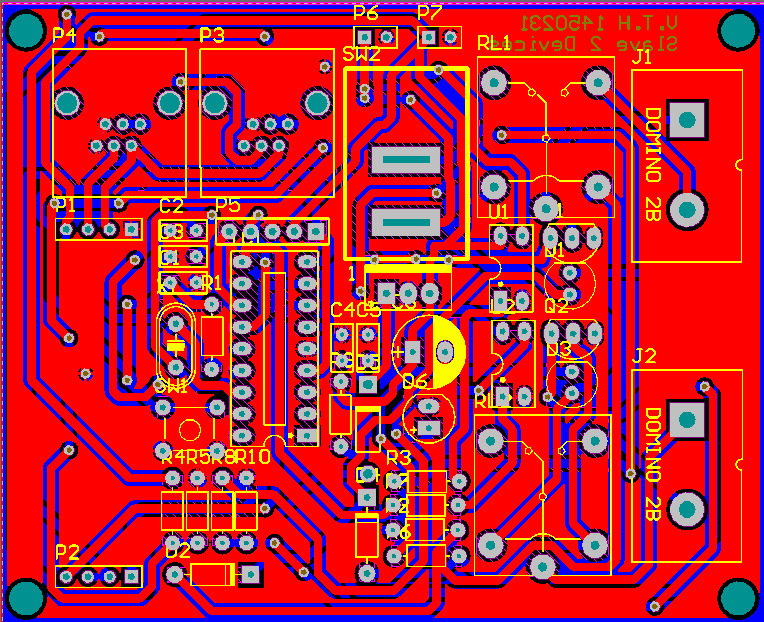
\includegraphics[scale=0.7]{images/s2rLayout.png}\\

    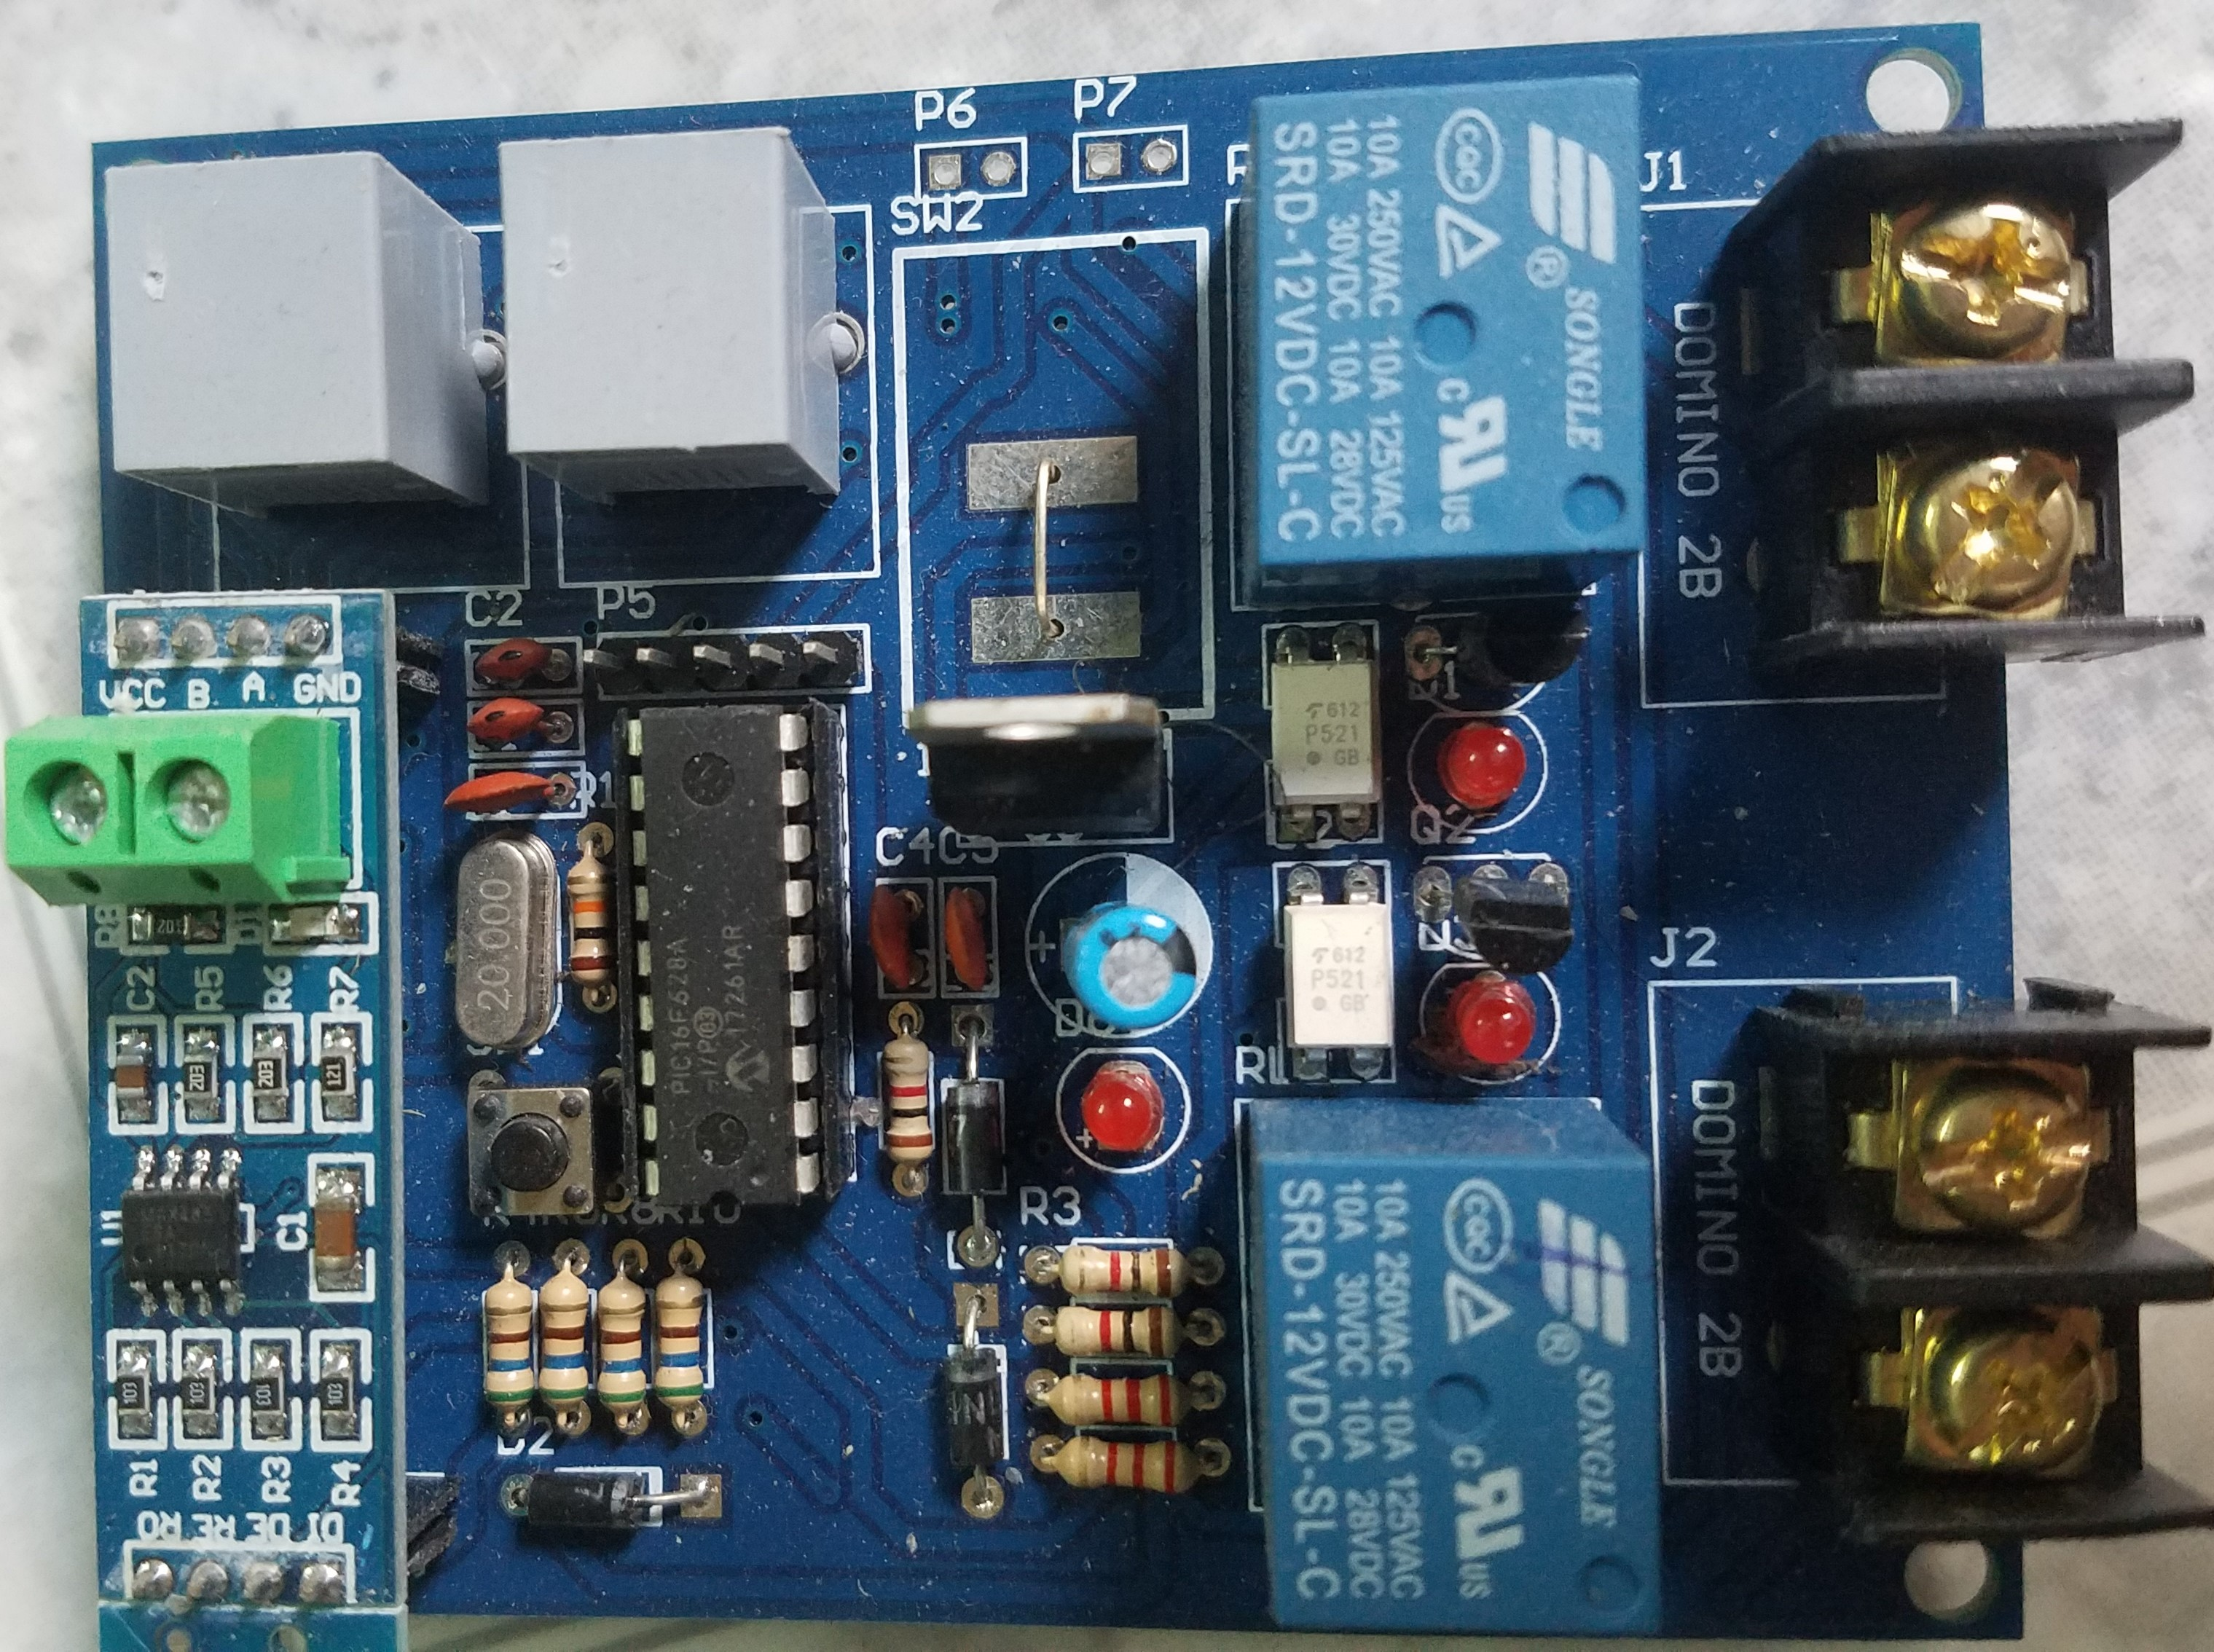
\includegraphics[scale=0.12]{images/s2r.jpg}
    \caption{Slave 2 Relays circuit}
    \label{fig:slave2RelaysCircuit}
    \end{center}
\end{figure}

\section{UI of Web Server}
This section presents the User Interface of the Web Server the author had introduced in previous chapter. Each Figure has its own caption to clarify the page title, in which can be match with the functions that were explained in previous chapter.
\begin{figure}[!ht]
    \begin{center}
    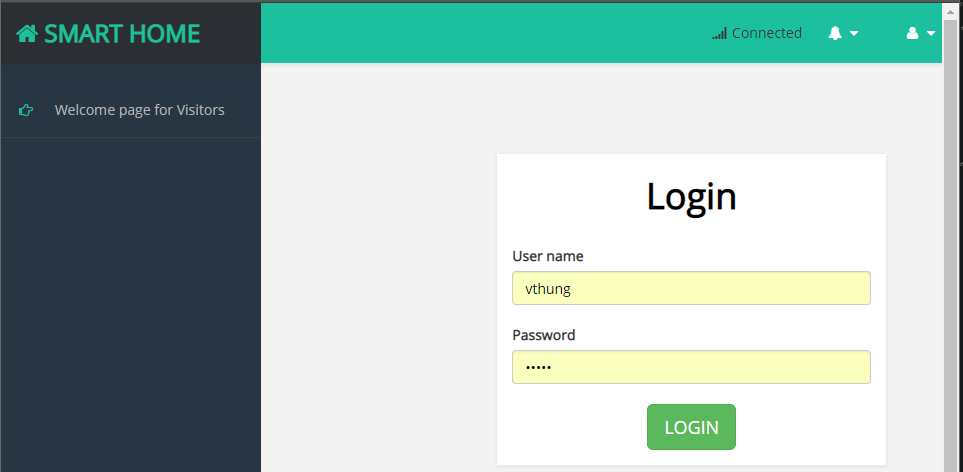
\includegraphics[scale=0.55]{images/login.png}
    \caption{Login page}
    \label{fig:login}
    \end{center}
\end{figure}
% \begin{figure}[!ht]
%     \begin{center}
%     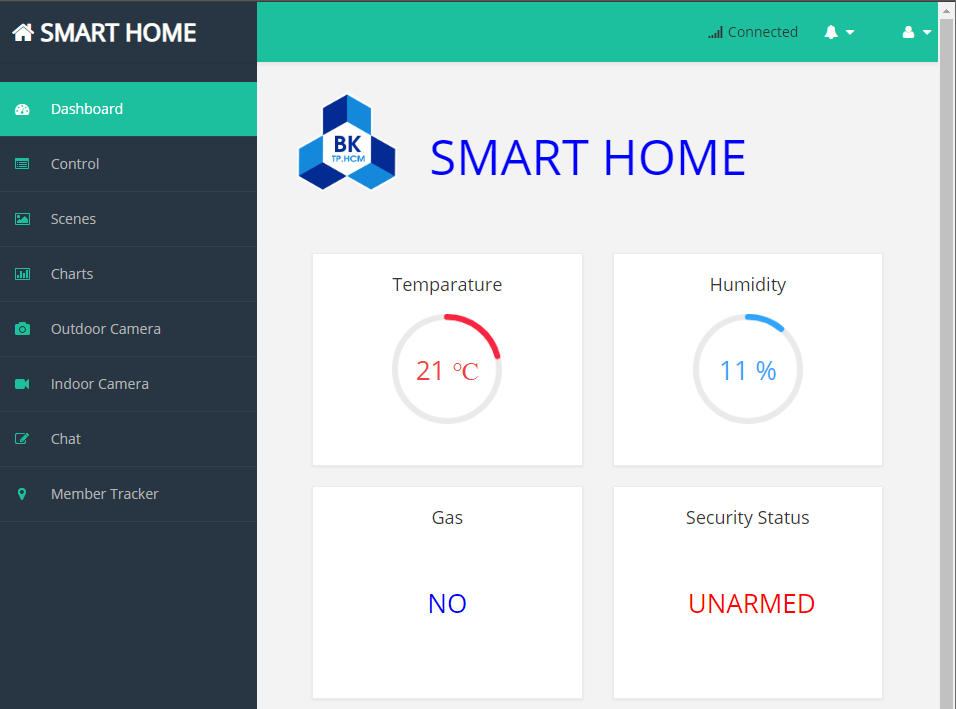
\includegraphics[scale=0.55]{images/dashboard.png}
%     \caption{Dashboard page}
%     \label{fig:dashboard}
%     \end{center}
% \end{figure}
\begin{figure}[!h]
    \begin{center}
    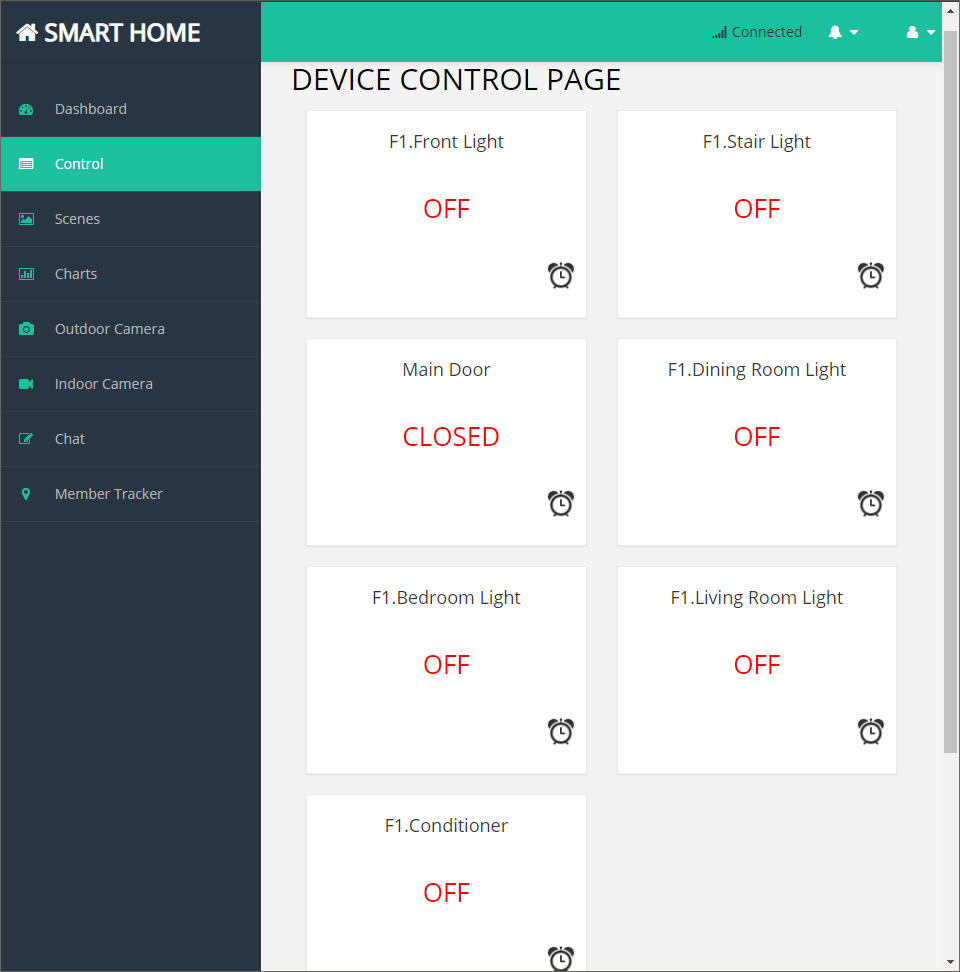
\includegraphics[scale=0.4]{images/control.png}
    \caption{Control page}
    \label{fig:control}
    \end{center}
\end{figure}
\begin{figure}[!ht]
    \begin{center}
    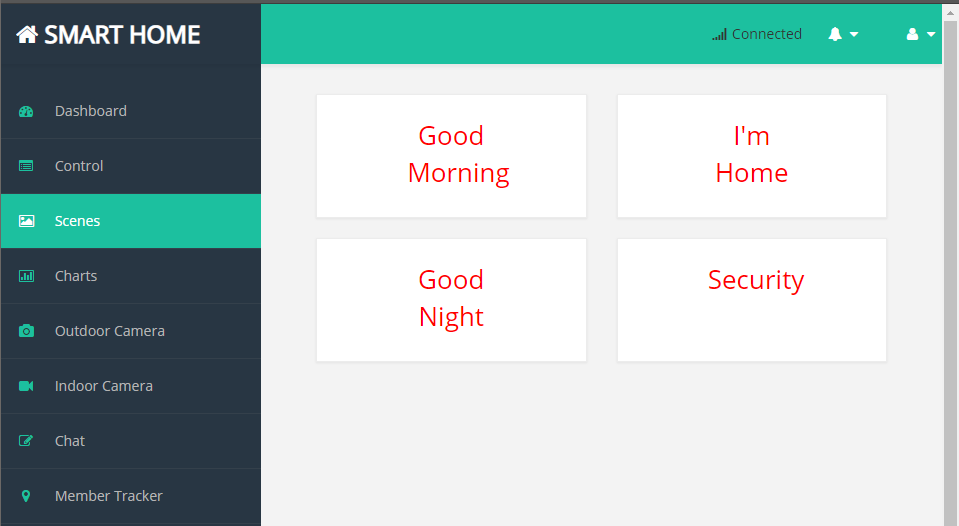
\includegraphics[scale=0.65]{images/scenario.png}
    \caption{Scenes page}
    \label{fig:scenario}
    \end{center}
\end{figure}
\begin{figure}[!ht]
    \begin{center}
    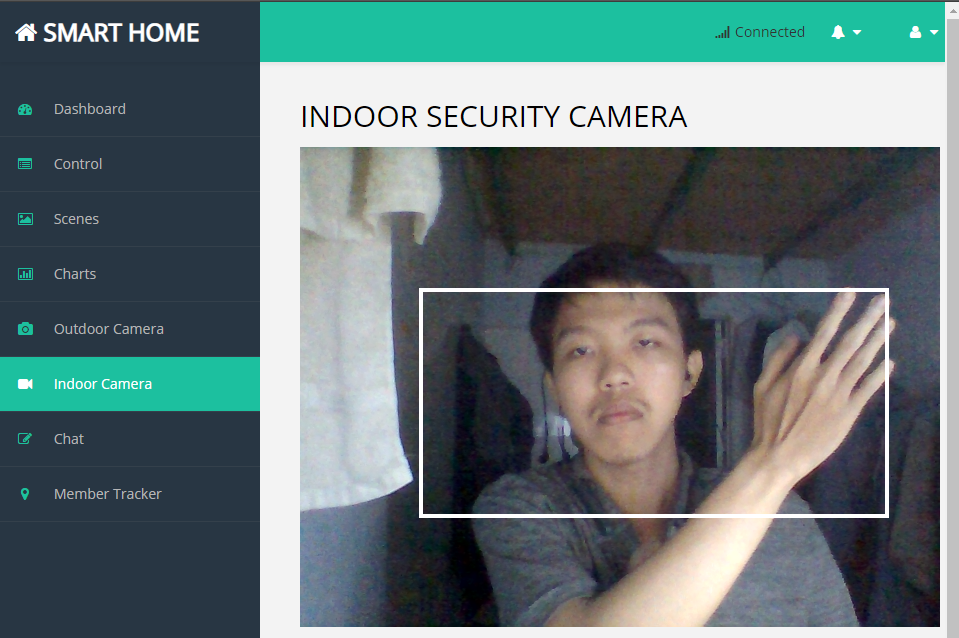
\includegraphics[scale=0.65]{images/indoor.png}
    \caption{Indoor Camera page}
    \label{fig:indoor}
    \end{center}
\end{figure}
\begin{figure}[!htbp]
    \begin{center}
    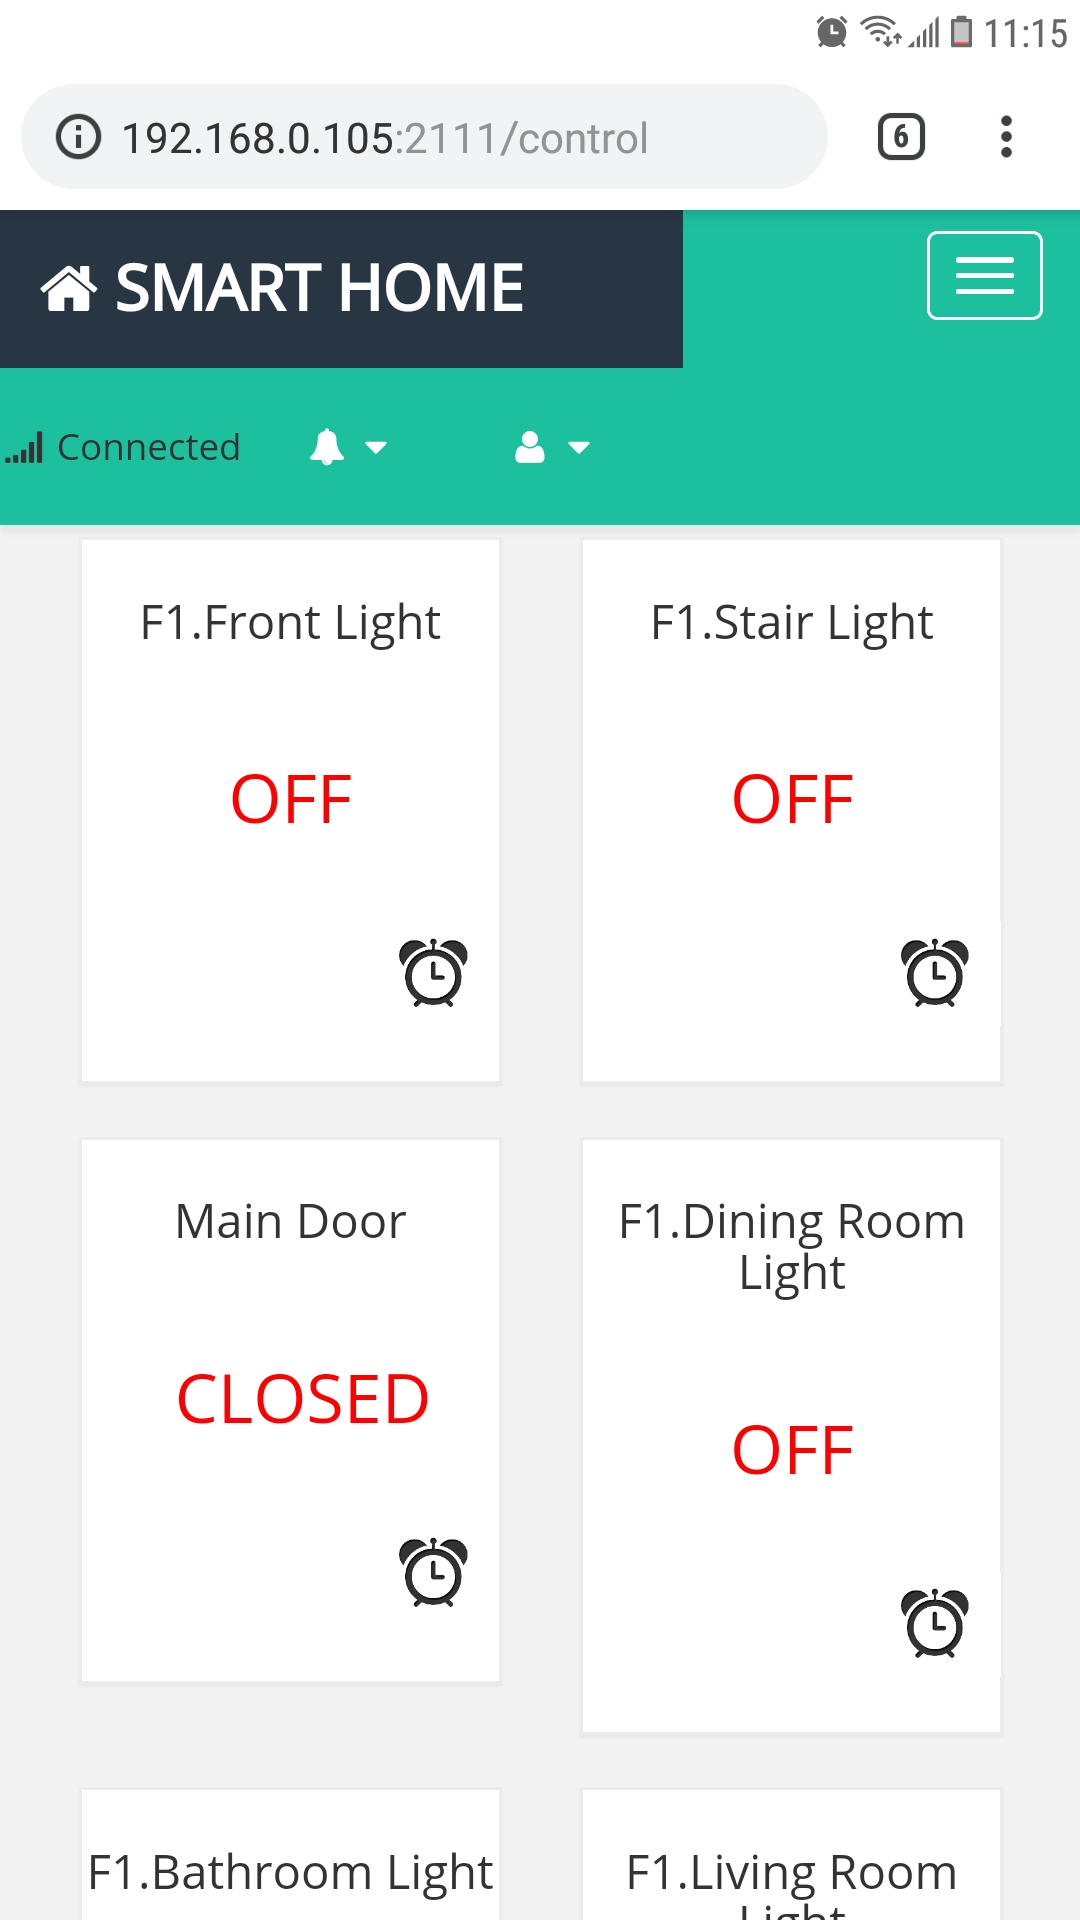
\includegraphics[scale=0.3]{images/controlOnCell.jpg}
    \caption{Control page on smart device with responsive website design}
    \label{fig:controlOnCell}
    \end{center}
\end{figure}
\begin{figure}[!htb]
    \begin{center}
    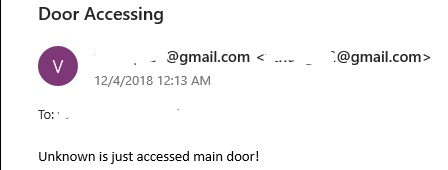
\includegraphics[scale=0.8]{images/doorAccess1.jpg}
    \caption{Door is Accessed by an Unknown person}
    \label{fig:doorAccess1}
    \end{center}
\end{figure}
\begin{figure}[!htb]
    \begin{center}
    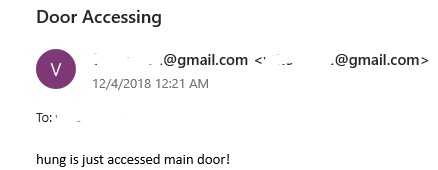
\includegraphics[scale=0.8]{images/doorAccess2.jpg}
    \caption{Door is Accessed by the owner}
    \label{fig:doorAccess2}
    \end{center}
\end{figure}
\begin{figure}[!htb]
    \begin{center}
    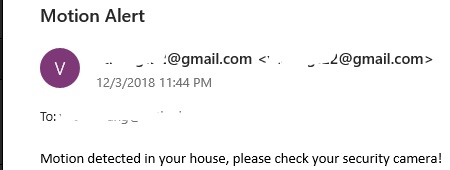
\includegraphics[scale=0.8]{images/emailAlert.jpg}
    \caption{Motion detected}
    \label{fig:emailAlert}
    \end{center}
\end{figure}
\begin{figure}[!htb]
    \begin{center}
    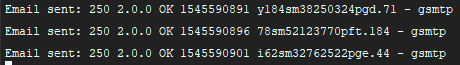
\includegraphics[scale=0.8]{images/emailSent.png}
    \caption{Announcement of sent email from command line}
    \label{fig:emailSent}
    \end{center}
\end{figure}

Refers from the Figure~\ref{fig:doorAccess1} to Figure~\ref{fig:emailSent}, they are the results of sent email to alert the owner in the event that any strange motion is detected while they are absent from the house. Furthermore, the access session of the Door is also alerted by email to the owner for them to keep track of the main entrance.

\section{UI and results of Security Camera Block}
Outdoor Security Camera Block is implemented in Raspberry Pi with a simple UI, which is illustrated with Figure~\ref{fig:rpiUi} is the main UI and Figure~\ref{fig:rpiAdminUi} is the interface to collect and train data. Also, the author shows the result of a recognized face with a small text is put beside with the rectangular ROI. However, the facial recognition system still, depends a lots on the environment condition, which leads to low rate of accuracy (about 70\% correct). The author’s intention is implementing the facial recognition with automatically open the main door after a face recognized. The processing speed is amazingly fast but it would make the thesis becomes more difficult to demonstrate, therefore, the system must be terminated by pressing ESC button on the keyboard. The result is shown with figure~\ref{fig:rpiCap}.
\begin{figure}[!htb]
    \begin{center}
    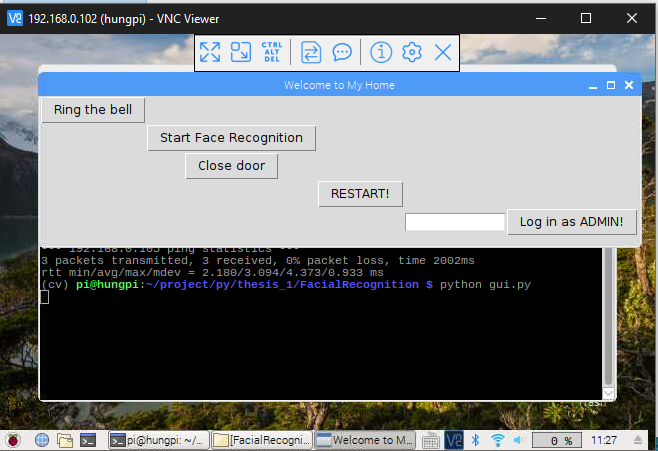
\includegraphics[scale=0.85]{images/rpiUi.png}
    \caption{Main UI of the software on Raspberry Pi}
    \label{fig:rpiUi}
    \end{center}
\end{figure}
\begin{figure}[!htb]
    \begin{center}
    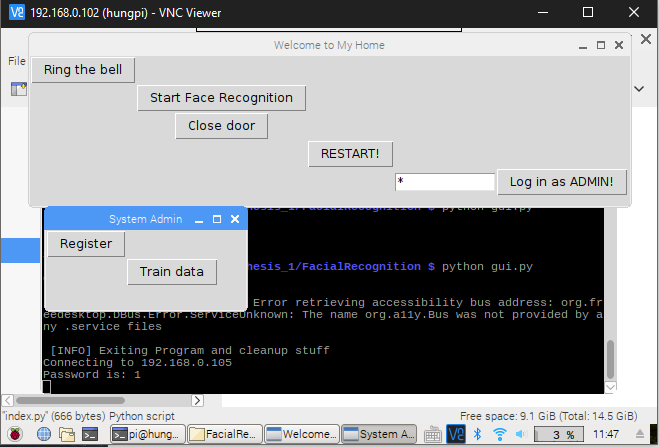
\includegraphics[scale=0.85]{images/rpiAdminUi.png}
    \caption{Admin UI of the pre-processing steps on Raspberry Pi}
    \label{fig:rpiAdminUi}
    \end{center}
\end{figure}
\begin{figure}[!htb]
    \begin{center}
    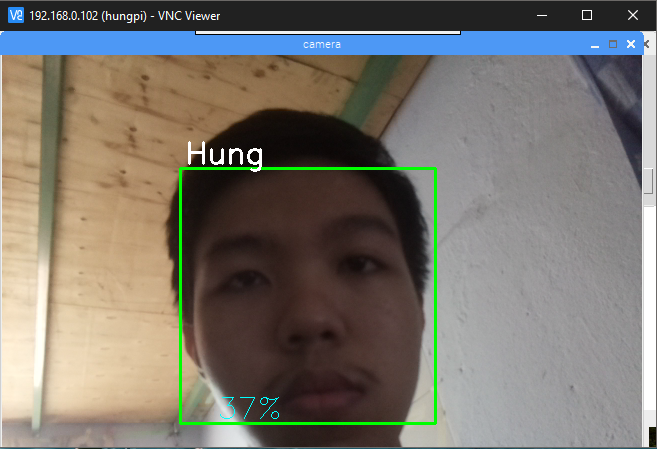
\includegraphics[scale=0.85]{images/rpiCap.png}
    \caption{Result of Facial Recognition function}
    \label{fig:rpiCap}
    \end{center}
\end{figure}